\documentclass[a4paper,twoside]{article}
\usepackage[T1]{fontenc}
\usepackage[bahasa]{babel}
\usepackage{graphicx}
\usepackage{graphics}
\usepackage{float}
\usepackage[cm]{fullpage}
\pagestyle{myheadings}
\usepackage{etoolbox}
\usepackage{algorithm}
\usepackage[noend]{algpseudocode}
\usepackage{setspace} 
\usepackage{lipsum} 
\usepackage{dirtree}
\usepackage{listings}
\usepackage{amsmath}
\usepackage{url}
\setlength{\headsep}{30pt}
\usepackage[inner=2cm,outer=2.5cm,top=2.5cm,bottom=2cm]{geometry} %margin
% \pagestyle{empty}
\newcommand{\appline}{
	\ifdefstring{\vmode}{final}{\renewcommand{\vlineno}{no}}{}
	\ifdefstring{\vlineno}{yes}{\linenumbers \def\linenumberfont{\normalfont\tiny\sffamily}}{}
	\ifdefstring{\vlineno}{no}{\lstset{numbers=left, stepnumber=1, numbersep=5pt}}{}
	
}
\makeatletter
\renewcommand{\@maketitle} {\begin{center} {\LARGE \textbf{ \textsc{\@title}} \par} \bigskip {\large \textbf{\textsc{\@author}} }\end{center} }
\renewcommand{\thispagestyle}[1]{}
\markright{\textbf{\textsc{Laporan Perkembangan Pengerjaan Skripsi\textemdash Sem. Ganjil 2015/2016}}}

\onehalfspacing
 
\begin{document}

\title{\@judultopik}
\author{\nama \textendash \@npm} 

%ISILAH DATA DATA BERIKUT INI:
\newcommand{\nama}{Ega Prianto}
\newcommand{\@npm}{2013730047}
\newcommand{\tanggal}{24/11/2016} %Tanggal pembuatan dokumen
\newcommand{\@judultopik}{Deteksi Gerakan Kepala dengan Google Cardboard} % Judul/topik anda
\newcommand{\kodetopik}{PAS4102}
\newcommand{\jumpemb}{1} % Jumlah pembimbing, 1 atau 2
\newcommand{\pembA}{Pascal Alfadian}
\newcommand{\pembB}{-}
\newcommand{\semesterPertama}{41 - Ganjil 16/17} % semester pertama kali topik diambil, angka 1 dimulai dari sem Ganjil 96/97
\newcommand{\lamaSkripsi}{1} % Jumlah semester untuk mengerjakan skripsi s.d. dokumen ini dibuat
\newcommand{\kulPertama}{Skripsi 1} % Kuliah dimana topik ini diambil pertama kali
\newcommand{\tipePR}{B} % tipe progress report :
% A : dokumen pendukung untuk pengambilan ke-2 di Skripsi 1
% B : dokumen untuk reviewer pada presentasi dan review Skripsi 1
% C : dokumen pendukung untuk pengambilan ke-2 di Skripsi 2
\maketitle

\pagenumbering{arabic}

\section{Data Skripsi} %TIDAK PERLU MENGUBAH BAGIAN INI !!!
Pembimbing utama/tunggal: {\bf \pembA}\\
Pembimbing pendamping: {\bf \pembB}\\
Kode Topik : {\bf \kodetopik}\\
Topik ini sudah dikerjakan selama : {\bf \lamaSkripsi} semester\\
Pengambilan pertama kali topik ini pada : Semester {\bf \semesterPertama} \\
Pengambilan pertama kali topik ini di kuliah : {\bf \kulPertama} \\
Tipe Laporan : {\bf \tipePR} -
\ifdefstring{\tipePR}{A}{
			Dokumen pendukung untuk {\BF pengambilan ke-2 di Skripsi 1} }
		{
		\ifdefstring{\tipePR}{B} {
				Dokumen untuk reviewer pada presentasi dan {\bf review Skripsi 1}}
			{	Dokumen pendukung untuk {\bf pengambilan ke-2 di Skripsi 2}}
		}

\section{Detail Perkembangan Pengerjaan Skripsi}
Detail bagian pekerjaan skripsi sesuai dengan rencan kerja/laporan perkembangan terkahir :
	\begin{enumerate}
		\item Melakukan studi literatur tentang Android SDK, Google VR SDK, Quaternion.\\
		{\bf status :} Ada sejak rencana kerja skripsi. Algoritma \textit{Head Motion Detection} tidak ditemukan literaturnya, algoritma dibuat pada bagian analisis metode pendeteksi gerakan kepala\\
		{\bf hasil :} 
		\begin{itemize}
			\item \textbf{Android SDK} 
		\end{itemize} 
		Dalam membuat aplikasi pada perangkat Android, dibutuhkan Android SDK. Android SDK(\textit{software development kit}) adalah kumpulan \textit{source code, development tools, emulator,}\cite{developers2011android} dan semua \textit{libraries} untuk membuat suatu aplikasi untuk \textit{platform} Android. IDE (\textit{integrated development environment} yang resmi untuk Android SDK adalah Android Studio. Android Studio dapat di download di halaman situs web Google Developer\cite{developers2011android}, sekaligus dengan Android SDKnya.  
				  
				\textbf{Struktur File Android Studio Project} 
				
				Pada saat project baru telah dibuat, Android Studio akan membuatkan folder-folder standar seperti pada Gambar \ref{fig:android-studio-structure}.
				\begin{figure}[htbp]
\dirtree{%
.1 {module}.
.2 {build} \ldots{} \begin{minipage}[t]{5cm}Folder yang mengandung file-file dari hasil pembangunan \textit{project}{.}\end{minipage}.
.2 {libs} \ldots{} \begin{minipage}[t]{5cm}Folder yang mengandung \textit{libraries} privat{.}\end{minipage}.
.2 {src} \ldots{} \begin{minipage}[t]{5cm}Folder yang mengandung semua kode dan file sumber untuk suatu modul{.}\end{minipage}.
.3 {androidTest} \ldots{} \begin{minipage}[t]{5cm}Folder yang mengandung kode untuk mengetes yang berjalan di perangkat Android{.}\end{minipage}.
.3 {main} \ldots{} \begin{minipage}[t]{5cm}Folder yang mengandung file-file kode dan file sumber inti dari suatu module{.}\end{minipage}.
.4 {AndroidManifest.xml} \ldots{} \begin{minipage}[t]{5cm}File yang mendeskripsikan sifat dari aplikasi dan setiap komponennya{.}\end{minipage}.
.4 {java} \ldots{} \begin{minipage}[t]{5cm}Folder yang mengandung kode-kode java{.}\end{minipage}.
.4 {jni} \ldots{} \begin{minipage}[t]{5cm}Folder yang mengandung kode-kode yang menggunakan Java Native Interface (JNI){.}\end{minipage}.
.4 {gen} \ldots{} \begin{minipage}[t]{5cm}Folder yang mengandung file-file java yang dihasilkan oleh Android Studio{.}\end{minipage}.
.4 {res} \ldots{} \begin{minipage}[t]{5cm}Folder yang mengandung file-file sumber untuk aplikasi, seperti file drawable, layout, dan UI String{.}\end{minipage}.
.4 {assets} \ldots{} \begin{minipage}[t]{5cm}Folder yang mengandung file yang akan di kompile menjadi file .apk{.}\end{minipage}.
.2 {build.gradle} \ldots{} \begin{minipage}[t]{5cm}File yang mendefinisikan konfigurasi modul untuk proses build{.}\end{minipage}.
.1 {build.gradle} \ldots{} \begin{minipage}[t]{5cm}File yang mendefinisikan konfigurasi proses build untuk project yang berlaku untuk semua modul{.}\end{minipage}.
}
				\caption{Tampilan struktur folder pada \textit{project} Android Studio}
				\label{fig:android-studio-structure}
				\end{figure}

				\textbf{Membuat Interface Android}\\
				
\cite{android_developers}
Pada bagian ini akan dijelaskan bagaimana membuat layout di XML termasuk \textit{text field} dan \textit{button}.\\

	 Hierarki \textit{Graphical User Interface} (GUI) untuk Aplikasi Android\\
		\label{sssec:hierarki_gui_untuk_aplikasi_android}
		
		GUI untuk aplikasi Android dibuat dengan hierarki dari objek View dan ViewGroup (Gambar \ref{fig:viewgroup}). Objek-objek dari View biasanya adalah \textit{UI(User Interface) Widgets} seperti \textit{button} atau \textit{text field}. Objek-objek dari ViewGroup tidak terlihat oleh \textit{view containers} yang mendefinisikan bagaimana \textit{child views} ditata seperti \textit{grid} atau \textit{vertical list}.

		\begin{figure}[htbp]
			\centering
				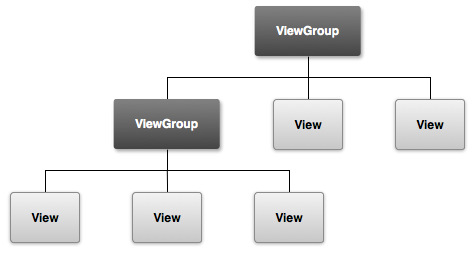
\includegraphics[scale=1]{Gambar/viewgroup.png}
			\caption{Illustrasi bagaimana percabangan objek ViewGroup pada \textit{layout} dan mengandung objek View lainnya.}
			\label{fig:viewgroup}
		\end{figure}

		Android menggunakan file XML yang berkorespondesi kepada \textit{subclasses} dari View dan ViewGroup, sehingga UI dapat didefinisikan dalam XML menggunakan hierarki dari elemen UI.\\

 Attribut-attribut Objek View\\

\label{sssec:attribut_attribut_objek_view}
Pada bagian ini akan dijelaskan attribut-attribut object View yang digunakan dalam membuat GUI pada file activity\_main.xml
\begin{itemize}
	\item \textbf{android:id}
	Attribut ini merupakan pengidentifikasi dari suatu view. Attribut ini dapat digunakan untuk menjadi referrensi object dari kode aplikasi seperti membaca dan memanipulasi objek tersebut (Akan dijelaskan lebih lanjut pada bagian Activity). Tanda '@' dibutuhkan ketika mereferensi object dari suatu XML. Tanda '@' tersebut diikuti dengan tipe (id pada kasus ini), \textit{slash}, dan nama (edit\_message pada Listing \ref{lst:attribute-view}). Tanda tambah (+) sebelum tipe hanya dibutuhkan jika ingin mendefinisikan \textit{resource ID} untuk pertama kalinya.
	\item \textbf{android:layout\_width} dan \textbf{android:layout\_height}
	Attribut ini digunakan untuk mendefinisikan panjang dan lebar dari suatu objek View. Daripada menggunakan besar spesifik untuk panjang dan lebarnya, lebih baik menggunakan "wrap\_content" yang menspesifikasi viewnya hanya akan sebesar yang dibutuhkan untuk memuat konten-konten dari View. Jika menggunakan "match\_parent" pada kasus Listing \ref{lst:attribute-view} View akan memenuhi layar, karena besarnya akan mengikuti besar dari paretnya LinearLayout.


	\item \textbf{android:hint}
	Attribut ini merupakan \textit{default string} untuk di tampilkan ketika objek View kosong. Daripada menggunakan \textit{hard-coded string} sebagai \textit{nilai} untuk ditampilkan, \textit{value} "@string/edit\_message" mereferensi ke sumber string pada file yang berbeda. Karena mereferensi ke sumber konkrit, maka tidak dibutuhkan tanda tambah (+). Nilai string ini akan di simpan pada file Strings.xml yang ditunjukkan pada Listing \ref{lst:string-xml}.
	\begin{lstlisting}[language=xml,numbers=left,breaklines=true,caption={Contoh kode pada string.xml},label={lst:string-xml},language=xml]
<resources>
	<string name="app_name">MyFirstAndroidApp</string>
	<string name="edit_message">Ini adalah hint</string>
	<string name="button_send">Send</string>
</resources>

\end{lstlisting}


	\item \textbf{android:onClick}
	Attribut ini akan memberitahu \textit{system} untuk memanggil method yang sesuai namanya (contoh pada Listing \ref{lst:attribute-view} adalah \textbf{sendMessage()}) di Activity ketika pengguna melakukan klik pada \textit{button} tersebut. Agar \textit{system} dapat memanggil method yang tepat, method tersebut harus memenuhi kriteria berikut.
	\begin{itemize}
		\item \textit{Access Modifier} haruslah \textit{public}.
		\item Harus \textit{void return value}nya.
		\item Mempunyai View sebagai parameter satu-satunya. View ini akan diisi dengan View yang di klik.
	\end{itemize}
\begin{lstlisting}[language=xml,numbers=left,breaklines=true,caption={Contoh kode file XML pada folder layout},label={lst:attribute-view},language=xml]
<LinearLayout
	xmlns:android="http://schemas.android.com/apk/res/android"
	xmlns:tools="http://schemas.android.com/tools"
	android:layout_width="match_parent"
	android:layout_height="match_parent"
	android:orientation="horizontal">
	<EditText android:id="@+id/edit_message"
			android:layout_weight="1"
			android:layout_width="0dp"
			android:layout_height="wrap_content"
			android:hint="@string/edit_message" />
	<Button
			android:layout_width="wrap_content"
			android:layout_height="wrap_content"
			android:text="@string/button_send"
			android:onClick="sendMessage" />
</LinearLayout>
\end{lstlisting}
\end{itemize}


\textbf{Activity}\\

\label{sec:activity}
\cite{android_developers}
Activity adalah suatu hal yang terfokuskan dengan apa yang bisa pengguna lakukan. Hampir semua \textit{Activity} berinteraksi dengan pengguna, jadi kelas Activity akan membuat suatu halaman baru yang bisa ditambahkan dengan konten-konten View. Selain dapat direpresentasikan kepada pengguna dengan halaman \textit{full-screen}, Activity juga dapat direpresentasikan dengan cara lain: seperti halaman \textit{floating} atau tertanam di Activity lain.\\

Activity Lifecycle\\

\label{sssec:activity_lifecycle}
\begin{figure}[htbp]
	\centering
		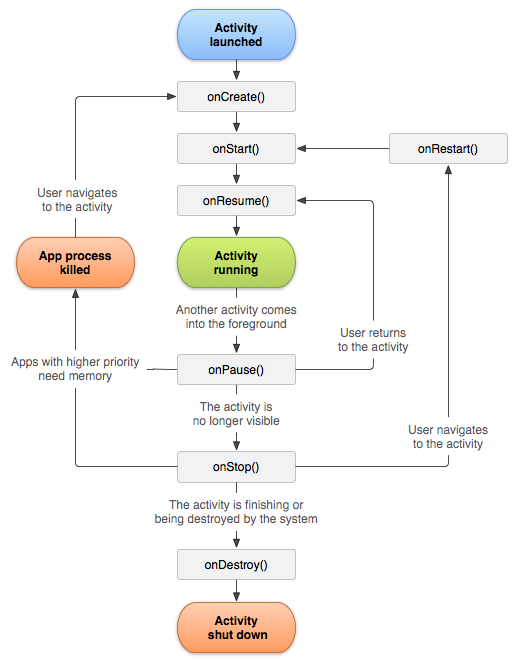
\includegraphics[scale=0.48]{Gambar/activity-lifecycle.png}
	\caption{\textit{State diagram} siklus Activity}
	\label{fig:activity-lifecycle}
\end{figure}

Aktivitas dalam sistem android di atur sebagai \textit{activity stack}. Ketika ada Activity baru yang dimulai, Activity tersebut ditempatkan di paling atas pada \textit{stack} dan menjadi Activity aktif. Activity sebelumnya akan tetap berada di bawah stack, dan tidak akan muncul lagi sampai Activity yang baru berakhir. 

Activity didasari dari empat kondisi:
\begin{itemize}
	\item Jika Activity berada di latar depan pada layar, Activity tersebut sedang aktif.
	\item Jika Activity sudah tidak terfokuskan tetapi masih dapat terlihat, Activity tersebut sedang berhenti sementara. Pada kondisi ini Activity tersebut masih berjalan, tapi bisa diberhentikan ketika system berada dalam situasi kekurangan memori.
	\item Jika suatu Activity benar-benar dihalangi oleh Activity lain, Activity tersebut telah berhenti. Activity tersebut akan tetap mengingat seluruh keadaan dan infomasi anggota tetapi, Activity tersebut tidak lagi terlihat oleh pengguna jadi tampilan jendelanya akan tersembunyi dan seringkali akan diberhentikan Activitynya ketika system membutuhkan memori.
	\item Jika suatu Activity sedang berhenti sementara atau berhenti total, sistem dapat membuang Activity dari memory dengan cara menanyakan kepada pengguna untuk memberhentikannya atau langsung diberhentikan oleh sistem. Jika Activity tersebut ditampilkan lagi kepada pengguna, Activity tersebut harus memulai dari awal dan kembali ke keadaan sebelumnya.
\end{itemize}
Gambar \ref{fig:activity-lifecycle} menunjukkan pentingnya alur keadaan dari suatu Activity. Gambar segi empat merepresentasikan \textit{callback methods} yang dapat diimplementasikan untuk melakukan operasi ketika Activity berubah kondisi. Oval berwarna merupakan kondisi-kondisi utama dari suatu Activity.
Ada 3 \textit{key loops} untuk memantau suatu Activity:
\begin{itemize}
	\item \textit{Entire lifetime} terjadi diantara pemanggilan pertama pada onCreate(Bundle) sampai ke satu pemanggilan akhir onDestroy(). Suatu Activity akan melakukan semua persiapan pada kondisi umum pada method onCreate(), dan melepaskan seluruh sisa pemrosesan pada method onDestroy().
	\item \textit{Visible lifetime} terjadi antara pemanggilan onStart() sampai pemanggilan yang sesuai pada onStop(). Pada tahap ini pengguna dapat melihat Activity pada layar meskipun tidak berada pada \textit{foreground} dan berinteraksi dengan pengguna.
	\item \textit{Foreground lifetime} terjadi antara pemanggilan method onResume() sampai ke satu pemanggilan akhir onDestroy(). Pada tahap ini Activity berada di depan semua Activity lainnya dan sedang berinteraksi dengan user.
\end{itemize}


\textbf{Android Sensor Framework}\\

\label{sec:android_sensor_framework}
\cite{android_developers}Sebagian besar dari perangkat android sudah memiliki sensor yang mengukur gerakan, orientasi, dan berbagai keadaan lingkungan. Sensor-sensor ini dapat memberikan data mentah dengan tingkat akurasi yang tinggi. Sensor ini juga berguna untuk memantau pergerakan tiga dimensi atau posisi perangkat. Sensor ini juga dapat memantau perubahan keadaan lingkungan yang dekat dengan perangkat. 
Android mendukung tiga kategori sensor:
\begin{itemize}
	\item \textbf{Sensor gerak}
	Sensor-sensor ini mengukur akselerasi dan rotasi pada tiga sumbu. Kategori sensor ini meliputi \textit{accelerometers}, sensor gravitasi, \textit{gyroscope}, dan \textit{rotation vector}. 
	\item \textbf{Sensor keadaan lingkungan}
	Sensor-sensor ini mengukur berbagai keadaan lingkungan seperti suhu udara, tekanan, pencahayaan, dan kelembaban. Kateori sensor ini termasuk barimeter, fotometer dan termometer.
	\item \textbf{Sensor posisi}
	Sensor-sensor ini mengukur posisi perangkat. Kategori sensor ini meliputi sensor orientasi dan magnetometer.
\end{itemize}
Android Sensor Framework membantu developers untuk mengakses berbagai jenis sensor. Beberapa sensor berbasis perangkat keras dan beberapa sensor berbasis perangkat lunak. Sensor berbasis perangkat keras mendapatkan data dengan langsung mengukur sifat lingkungan tertentu, seperti percepatan, kekuatan medan geomagnetik, atau perubahan sudut. Sensor berbasis perangkat lunak mendapatkan data dari satu atau lebih sensor berbasis perangkat keras. Sensor berbasis perangkat lunak ini juga terkadang disebut sensor virtual atau sensor sintetis. Pada tabel berikut akan dirincikan tipe-tipe setiap sensor posisi dan gerak, deskripsi, dan penggunaan umumnya.

\begin{table}[htbp]
	\centering
	\caption{Tipe-tipe Sensor pada Android}
\begin{tabular}{|p{6.3cm}| p{1.5cm}| p{5cm}| p{2.4cm}|} 
\hline
Sensor & Tipe & Deskripsi & Penggunaan umum\\ \hline
TYPE\_ACCELEROMETER & Perangkat Keras & Mengukur percepatan dalam \(m/s^2\) yang terjadi pada perangkat di semua tiga sumbu fisik (x,y,z), termasuk percepatan gravitasi. & Deteksi gerak(goncangan, keseimbangan, dan lain-lain)\\ \hline
TYPE\_GRAVITY & Perangkat Lunak atau Perangkat Keras & Mengukur percepatan gravitasi dalam \(m/s^2\) yang terjadi pada perangkat di tiga sumbu fisik (x,y, dan z) & Deteksi gerak(goncangan, keseimbangan, dan lain-lain)\\ \hline
TYPE\_GYROSCOPE & Perangkat Keras & Mengukur rata-rata rotasi sudut dalam \(rad/s\) di tiga sumbu fisik (x,y, dan z). & Deteksi rotasi (putaran, belokan, dan lain-lain).\\ \hline
TYPE\_LINEAR\_ACCELERATION & Perangkat Lunak atau Perangkat Keras & Mengukur percepatan dalam \(m/s^2\) yang terjadi pada perangkat di semua tiga sumbu fisik (x,y,z), tidak termasuk percepatan gravitasi. & Memantau percepatan pada suatu sumbu.\\ \hline
TYPE\_MAGNETIC\_FIELD & Perangkat Keras & Mengukur medan magnet sekitar untuk semua tiga sumbu fisik (x,y, dan z) di satuan \(\mu T\). & Membuat Kompas.\\ \hline
TYPE\_ORIENTATION & Perangkat Lunak & Mengukur derajat rotasi yang terjadi pada perangkat pada semua tiga sumbu fisik (x,y, dan z). & Menentukan posisi perangkat \\ \hline
TYPE\_ROTATION\_VECTOR & Perangkat Lunak dan Perangkat Keras & Mengukur orisentasi dari suatu perangkat dengan menyediakan tiga element dari vektor rotasi perangkat. & Deteksi gerak dan deteksi rotasi.\\ \hline
\end{tabular}
\end{table}

Sistem Koordinat Sensor\\

\label{sssec:sistem_koordinat_sensor}
Pada umumnya, sensor framework menggunakan sistem tiga sumbu koordinat standar untuk mengekspresikan nilai data. Sebagian besar sensor sistem koordinat didefinisikan relatif terhadap layar perangkat bila perangkat dibuat dalam orientasi standar (lihat Gambar \ref{fig:axis-device})
\begin{figure}[htbp]
	\centering
		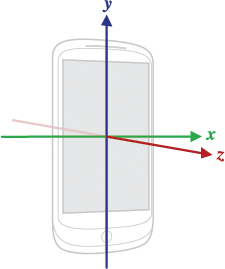
\includegraphics[scale=1]{Gambar/axis-device.png}
	\caption{Sistem koordinat (relatif dengan perangkatnya) yang digunakan oleh Sensor API}
	\label{fig:axis-device}
\end{figure}
Sensor-sensor yang menggunakan sistem tiga sumbu seperti Gambar \ref{fig:axis-device} adalah sebagai berikut :
\begin{itemize}
	\item Accelerometer
	\item Sensor Gravitasi
	\item Gyroscope
	\item Sensor Percepatan Linear
	\item Sensor Medan Geomagnetik
\end{itemize}
Koordinat sistem yang sumbunya tidak tertukar ketika orientasi perangkat berubah. Sistem koordinat sensor tidak pernah berubah seiring perangkatnya bergerak. Dalam aplikasi android tidak dapat diassumsikan bahwa standar orientasi perangkat android adalah \textit{portrait}. Kebanyakan perangkat \textit{Tablet} standar orientasinya adalah \textit{landscape}. Sistem koordinat sensor selalu di dasarkan pada orientasi dasar dari suatu perangkat android.\\

Mengidentifikasi Sensor dan Kapabilitas Sensor\\

\label{sssec:mengidentifikasi_sensor_dan_kapabilitas_sensor}
Android Sensor Framework menyediakan beberapa method yang dapat membuat developer mudah untuk menentukan sensor mana yang akan digunakan. APInya juga dapat menyediakan method yang memungkinkan penggunanya menentukan kapabilitas masing-masing sensor, seperti jangkauan maksimum, resolusi, dan kebutuhan dayanya.
Untuk mengidentifikasi sensor-sensor yang ada pada perangkat, hal pertama yang perlu dilakukan adalah mendapatkan referensi sensor tersebut. Untuk mendapatkan referensi tersebut, dapat dilakukan dengan membuat instansiasi dari kelas SensorManager dan memanggul method getSystemService() dan memasukkan isi Parameternya dengan SENSOR\_SERVICE. Contohnya pada Listing \ref{lst:init-sensor-manager}.
 
\begin{lstlisting}[language=java,numbers=left,breaklines=true,caption={Contoh inisialisasi kelas SensorManager},label={lst:init-sensor-manager},language=java]
private SensorManager mSensorManager;
...
mSensorManager = (SensorManager) getSystemService(Context.SENSOR_SERVICE);
\end{lstlisting}

Kemudian untuk mendapatkan daftar dari setiap sensor pada suatu perangkat dapat dilakukan dengan cara memanggil method getSensorList() dan menggunakan konstanta TYPE\_ALL pada kelas Sensor. Contohnya pada Listing \ref{lst:get-sensor-lists}

\begin{lstlisting}[language=java,numbers=left,breaklines=true,caption={Contoh untuk mendapatkan daftar dari setiap sensor yang ada},label={lst:get-sensor-lists},language=java]
List<Sensor> deviceSensors = mSensorManager.getSensorList(Sensor.TYPE_ALL);
\end{lstlisting}

Namun jika ingin mendapatkan sensor-sensor yang sesuai dengan tipe sensor yang diberikan, dapat menggunakan TYPE\_GYROSCOPE, TYPE\_LINEAR\_ACCELERATION, TYPE\_GRAVITY, atau TYPE\_GRAVITY.

Untuk menentukan jenis tertentu dari sensor yang ada pada perangkat dapat didapatkan dengan method getDefaultSensor() dengan dimasukkan dengan konstanta yang berada pada kelas Sensor. Jika perangkatnya memiliki lebih dari satu sensor dari tipe sensor yang diberikan, salah satu dari sensor tersebut akan dianggap sebagai sensor dasar. Jika sensor dasanya tidak ada untuk sensor tersebut, perangkat tersebut berarti tidak memiliki sensor dengan jenis yang diberikan. Listing \ref{lst:check-sensor} adalah contoh untuk mengecek apakah perangkat yang digunakan memiliki sensor dengan jenis yang diberikan.

\begin{lstlisting}[language=java,numbers=left,breaklines=true,caption={Contoh untuk mengecek apakah perangkat yang digunakan memiliki sensor dengan jenis yang diberikan},label={lst:check-sensor},language=java]
private SensorManager mSensorManager;
...
mSensorManager = (SensorManager) getSystemService(Context.SENSOR_SERVICE);
if (mSensorManager.getDefaultSensor(Sensor.TYPE_MAGNETIC_FIELD) != null){
// Sukses! Perangkat ini memiliki sensor magnetometer.
}
else {
// Gagal! Perangkat ini tidak memiliki sensor magnetometer.
}
\end{lstlisting}

Jika ingin membatasi versi atau vendor dari sensor yang akan digunakan, dapat menggunakan method getVendor() dan getVersion(). Seperti pada Listing \ref{lst:check-sensor-version} yang mengharuskan sensor gravitasi bervendor "Google Inc." dan memiliki versi 3. Jika sensor tersebut tidak tersedia pada perangkat, sensor accelerometerlah yang digunakan.

\begin{lstlisting}[language=java,numbers=left,breaklines=true,caption={Contoh untuk mengecek apakah perangkat yang digunakan memiliki sensor dengan jenis yang diberikan},label={lst:check-sensor-version},language=java]
private SensorManager mSensorManager;
private Sensor mSensor;

...

mSensorManager = (SensorManager) getSystemService(Context.SENSOR_SERVICE);
mSensor = null;

if (mSensorManager.getDefaultSensor(Sensor.TYPE_GRAVITY) != null){
  List<Sensor> gravSensors = mSensorManager.getSensorList(Sensor.TYPE_GRAVITY);
  for(int i=0; i<gravSensors.size(); i++) {
    if ((gravSensors.get(i).getVendor().contains("Google Inc.")) &&
       (gravSensors.get(i).getVersion() == 3)){
      // menggunakan sensor gravitasi versi 3.
      mSensor = gravSensors.get(i);
    }
  }
}
if (mSensor == null){
  // Use the accelerometer.
  if (mSensorManager.getDefaultSensor(Sensor.TYPE_ACCELEROMETER) != null){
    mSensor = mSensorManager.getDefaultSensor(Sensor.TYPE_ACCELEROMETER);
  }
  else{
    // Tidak ada sensor gravitasi dan sensor accelerometer!
  }
}
\end{lstlisting}

Salah satu method yang sangat berguna lagi adalah, getMinDelay(). Method ini digunakan untuk mengetahui minimum interval waktu suatu sensor dapat menerima data dalam mikrodetik. Jika method getMinDelay() mengembalikan nilai nol, hal ini berarti sensor ini akan mengembalikan data setiap kali ada perubahan nilai pada sensor tersebut. 

Memonitor Nilai Sensor\\

\label{sssec:memonitor_nilai_sensor}

Untuk memonitor data mentah dari sensor, dibutuhkan untuk mengimplement dua buah method callback yang berada pada interface SensorEventListener. Kedua method tersebut adalah onAccuracyChanged(Sensor sensor, int accuracy) dan onSensorChanged(SensorEvent event). Sistem android akan memanggil kedua method ini ketika terjadi salah satu kondisi ini:

\begin{itemize}
	\item \textbf{Perubahan akurasi sensor.}\\
Dalam kasus ini sistem memanggil method onAccuracyChanged(Sensor sensor, int accuracy). Parameter sensor akan diberikan objek Sensor yang telah berubah akurasinya, dan parameter accuracy adalah nilai akurasi sensor yang baru.
	\item \textbf{Sensor memberitahu adanya nilai baru.}\\
Dalam kasus ini sistem memanggil method onSensorChanged(SensorEvent event), dengan parameter event akan diisi dengan objek SensorEvent untuk mendapatkan nilai barunya. Objek SensorEvent Mengandung semua infromasi tentang data sensor yang baru, termasuk: akurasi dari data, sensor yang mendapatkan data, dan catatan waktu data tersebut didapatkan, dan data yang baru yang telah didapatkan.
\end{itemize}

Pada Listing \ref{lst:monitoring-light-sensor} akan ditunjukkan bagaimana menggunakan method onSensorChanged(SensorEvent event) untuk memonitor data dari sensor cahaya. Pada Listing \ref{lst:monitoring-light-sensor} akan menampilkan data mentah dari sensor ke TextView yang telah didefinisikan pada file main.xml sebagai sensor\_data.
\begin{lstlisting}[language=java,numbers=left,breaklines=true,caption={Contoh memonitor data mentah pada sensor cahaya},label={lst:monitoring-light-sensor},language=java]
public class SensorActivity extends Activity implements SensorEventListener {
  private SensorManager mSensorManager;
  private Sensor mLight;

  @Override
  public final void onCreate(Bundle savedInstanceState) {
    super.onCreate(savedInstanceState);
    setContentView(R.layout.main);

    mSensorManager = (SensorManager) getSystemService(Context.SENSOR_SERVICE);
    mLight = mSensorManager.getDefaultSensor(Sensor.TYPE_LIGHT);
  }

  @Override
  public final void onAccuracyChanged(Sensor sensor, int accuracy) {
    // Hal yang perlu dilakukan aplikasi ketika akurasinya berubah.
  }

  @Override
  public final void onSensorChanged(SensorEvent event) {
    // Sensor cahaya akan mengembalikan 1 nilai saja.
    // Banyak sensor lain yang akan mengembalikan lebih dari 1 nilai.
    float lux = event.values[0];
    // Hal yang perlu dilakukan ketika ada perubahan data.
  }

  @Override
  protected void onResume() {
    super.onResume();
    mSensorManager.registerListener(this, mLight, SensorManager.SENSOR_DELAY_NORMAL);
  }

  @Override
  protected void onPause() {
    super.onPause();
    mSensorManager.unregisterListener(this);
  }
}
\end{lstlisting}
Pada method onSensorChanged(SensorEvent event), struktur nilai-nilai yang dikembalikan akan dijelaskan pada bagian Struktur Nilai yang Dikembalikan oleh Sensor. Pada method onResume(), ada pemanggilan method registerListener(). Method registerListener() ini berguna untuk menspesifikasikan waktu delay pada pemanggilan onSensorChanged(). Untuk menspesifikasikan delaynya dapat menggunakan konstanta yang ada pada kelas SensorManager. Konstanta-konstanta tersebut adalah SENSOR\_DELAY\_NORMAL (200.000 mikrodetik),SENSOR\_DELAY\_GAME (20.000 mikrodetik),SENSOR\_DELAY\_UI (60.000 mikrodetik), atau SENSOR\_DELAY\_FASTEST (0 mikrodetik). Pengaturan dasar untuk waktu delay ini menggunakan konstanta SENSOR\_DELAY\_NORMAL.
Perlu diperhatikan juga pemesanan sensor ketika activity sedang di berhentikan sementara maupun dilanjutkan kembali. Sistem tidak boleh tetap merekam sensor ketika activity tidak aktif. Hal ini diperlukan karena pada saat perangkat android menggunakan sensor, perangkat akan menggunakan tenanga yang banyak. Akan lebih baik jika penggunaan sensor diberhentikan ketika activitynya sudah tidak lagi digunakan. \\

Struktur Nilai yang Dikembalikan oleh Sensor\\

\label{sssec:struktur_nilai_yang_dikembalikan_oleh_sensor}
Setiap sensor android akan mengembalikan nilai-nilainya dengan struktur-struktur tertentu. Pada bab ini akan dijelaskan secara detil struktur nilai sistem android dalam mengembalikan nilai-nilai yang diperoleh dari sensor. Nilai ini akan didapatkan dengan tipe data array of float. Besar dan isi dari array tergantung pada sensor yang sedang di pantau. Berikut ini adalah struktur-struktur nilai dari setiap sensor pada sistem android :\\
\begin{itemize}
	\item \textbf{TYPE\_ACCELEROMETER}\\
Semua nilai didefinisikan sebagai satuan \(m/s^2\)
\begin{itemize}
	\item values[0]: Percepatan yang terjadi pada sumbu x dikali -1
	\item values[1]: Percepatan yang terjadi pada sumbu y dikali -1
	\item values[2]: Percepatan yang terjadi pada sumbu z dikali -1
\end{itemize}
Sensor ini mengukur percepatan(\(Ad\)) yang diterapkan pada perangkat. Sensor tersebut dapat mengukur percepatan dengan mengukur gaya(\(Fs\)) yang terjadi pada sensor menggunakan relasi berikut:
\[
	Ad = -\Sigma Fs / mass
\]
Secara khusus, gravitasi selalu mempengaruhi percepatan yang diukur :
\[
	Ad =  -g -\Sigma F / mass
\]
Karena inilah ketika perangkat android sedang diam, accelerometer membaca percepatan gravitasi sebesar \(g = 9.81m/s^2\).
Demikian pula ketika perangkat android sedang dalam keadaan jatuh bebas. Perangkat akan mempercepat menuju ke tanah pada percepatan \(9.81 m/s^2\), sehingga accelerometer membaca percepatan total sebesar \( 0 m/s^2\). 
Suatu saat akan di butuhkan untuk mengukur percepatan asli yang terjadi pada perangkat, sehingga kontribusi gravitasi harus di eliminasi. Hal ini bisa dilakukan dengan menerapkan \textit{high-pass} filter. Sebaliknya, \textit{low-pass} filter dapat digunakan untuk mendapatkan nilai gravitasi saja. 
\begin{lstlisting}[language=java,numbers=left,breaklines=true,caption={Implementasi \textit{low-pass} filter},label={lst:low-pass-filter},language=java]
public void onSensorChanged(SensorEvent event)
{
		// alpha dikalkulasikan sebagai t / (t + dT)
		// dengan t adalah low-pass filter's time-constant
		// dan dT, rata-rata event tersampaikan

		final float alpha = 0.8;

		gravity[0] = alpha * gravity[0] + (1 - alpha) * event.values[0];
		gravity[1] = alpha * gravity[1] + (1 - alpha) * event.values[1];
		gravity[2] = alpha * gravity[2] + (1 - alpha) * event.values[2];

		linear_acceleration[0] = event.values[0] - gravity[0];
		linear_acceleration[1] = event.values[1] - gravity[1];
		linear_acceleration[2] = event.values[2] - gravity[2];
}
\end{lstlisting}
\textit{Low-pass} filter dapat diimplementasikan pada Listing \ref{lst:low-pass-filter}\\
\item \textbf{TYPE\_MAGNETIC\_FIELD}\\
Sensor ini mengukur medan magnet sekitar perangkat pada sumbu X,Y, dan Z dalam satuan micro-Tesla.\\
\item \textbf{TYPE\_GYROSCOPE}\\
Sensor ini mengukur rata-rata perputaran pada perangkat yang berputar di sumbu X,Y, dan Z dalam satuan radians/second. Sistem koordinat yang digunakan sama dengan sistem koordinat pada sensor percepatan(Accelerometer). Jika perangkat berputar berlawanan arah jarum jam pada sumbu tertentu, maka rotasi yang terjadi akan bernilai positif. Perhatikan bahwa standar perputaran ini adalah definisi matematika standar pada rotasi positif.
\begin{itemize}
	\item values[0]: Percepatan angular pada sumbu X.
	\item values[1]: Percepatan angular pada sumbu Y.
	\item values[2]: Percepatan angular pada sumbu Z.
\end{itemize}
Biasanya keluaran dari gyroscope terintegrasi dari waktu ke waktu untuk menghitung rotasi yang menggambarkan perubahan sudut atas langkah waktu, misalnya pada Listing \ref{lst:gryoscope-example}

\begin{lstlisting}[language=java,numbers=left,breaklines=true,caption=contoh implementasi gyroscope,label={lst:gryoscope-example}]
private static final float NS2S = 1.0f / 1000000000.0f;
private final float[] deltaRotationVector = new float[4]();
private float timestamp;

public void onSensorChanged(SensorEvent event) {
// Pada tahapan ini delta rotasi akan dikalikan dengan rotasi saat ini
// setelah mengomputasinya dari data gyro.
	if (timestamp != 0) {
		final float dT = (event.timestamp - timestamp) * NS2S;
		// Sumbu dari rotasi, masih belum di normalisasi.
		float axisX = event.values[0];
		float axisY = event.values[1];
		float axisZ = event.values[2];

		// Menghitung percepatan angular
		float omegaMagnitude = sqrt(axisX*axisX + axisY*axisY + axisZ*axisZ);

		// Normalisasi rotasi vektor jika cukup besar untuk mendapatkan sumbunya.
		if (omegaMagnitude > EPSILON) {
				axisX /= omegaMagnitude;
				axisY /= omegaMagnitude;
				axisZ /= omegaMagnitude;
		}
		
		float thetaOverTwo = omegaMagnitude * dT / 2.0f;
		float sinThetaOverTwo = sin(thetaOverTwo);
		float cosThetaOverTwo = cos(thetaOverTwo);
		deltaRotationVector[0] = sinThetaOverTwo * axisX;
		deltaRotationVector[1] = sinThetaOverTwo * axisY;
		deltaRotationVector[2] = sinThetaOverTwo * axisZ;
		deltaRotationVector[3] = cosThetaOverTwo;
	}
}
timestamp = event.timestamp;
float[] deltaRotationMatrix = new float[9];
SensorManager.getRotationMatrixFromVector(deltaRotationMatrix, deltaRotationVector);
// User code should concatenate the delta rotation we computed with the current rotation
// in order to get the updated rotation.
// rotationCurrent = rotationCurrent * deltaRotationMatrix;
}

\end{lstlisting}
Dalam prakteknya, gyroscope \textit{noise} dan \textit{offset} akan menyebabkan beberapa kesalahan yang harus dikompensasi. Cara untuk mengkompensasinya biasanya dilakukan dengan menggunakan informasi dari sensor lain.\\
\item \textbf{TYPE\_GRAVITY}\\
Sensor ini menunjukkan arah dan besarnya vektor gaya gravitasi. Sensor ini mengembalikan nilai dengan satuan \(m/s^2\). Sistem koordinat sama seperti sistem koordinat yang umum digunakan sensor percepatan. 

Catatan: Bila perangkat sedang diam, maka keluaran dari sensor gravitasi harus identik dengan accelerometer. \\

\item \textbf{TYPE\_LINEAR\_ACCELERATION}\\
Sensor yang menunjukkan percepatan pada setiap sumbu perangkat, tidak termasuk percepatan yang terjadi karena gravitasi. Nilai diberikan dalam satuan \(m/s^2\). Sistem koordinat yang digunakan sama seperti sistem koordinat yang digunakan sensor percepatan. Keluaran dari sensor accelerometer, gravitasi dan percepatan linear harus mengikuti aturan berikut:
\[
	percepatan = gravitasi + percepatan linear
\]\\

\item \textbf{TYPE\_ORIENTATION}\\
Semua nilai adalah sudut dalam derajat.
\begin{itemize}
	\item values[0]: Azimuth, sudut diantara arah magnetik utara dengan sumbu y, sekitar sumbu z (0 sampai 359). 0 = Utara, 90 = Timur, 180 = Selatan, 270 = Barat
	\item values[1]: Pitch, rotasi sekitar sumbu x (-180 sampai 180), dengan nilai positif ketika sumbu x bergerak menuju sumbu y.
	\item values[2]: Roll, perputaran sekitar sumbu y (-90 sampai 90) pada kondisi potrait, sensor akan bernilai 0. Pada kondisi landscape ke kanan sensor akan bernilai 90 dan sebaliknya yaitu kondisi landscape ke kiri sensor akan bernilai -90.
\end{itemize}

Catatan: Definisi ini berbeda dengan definisi yaw, pitch, dan roll yang digunakan pada aviasi yang sumbu X adalah sepanjang sisi bidang.

Catatan: Sensor ini sudah tidak digunakan lagi(deprecated), yang digunakan sekarang adalah sensor rotasi vector.\\
\item \textbf{TYPE\_ROTATION\_VECTOR}\\
Sensor ini merepresentasikan orientasi perangkat dengan kombinasi dari sumbu dan sudut. Perangkat akan di putar sebesar sudut \(\theta\) mengelilingi sumbu \(x,y,z\). Tiga elemen dari vektor rotasi adalah (\(x \sin (\frac{\theta}{2}), y \sin (\frac{\theta}{2}), z \sin (\frac{\theta}{2})\)), sehingga besarnya vektor rotasi sama dengan \(\sin (\frac{\theta}{2})\), dan arah vektor rotasi sama dengan sumbu rotasi. Tiga elemen dari vektor rotasi sama dengan tiga komponen terakhir pada unit kuaternion(\(\cos (\frac{\theta}{2}),x \sin (\frac{\theta}{2}), y \sin (\frac{\theta}{2}), z \sin (\frac{\theta}{2})\)) yang dijelaskan pada bagian Teori Kuaternion. Elemen dari vektor rotasi tak memiliki satuan. Sistem koordinat yang digunakan sama dengan sistem koordinat yang digunakan pada sensor percepatan. Referensi koordinat didefinisikan sebagai basis orthonormal, yaitu:
\begin{itemize}
	\item X didefinisikan sebagai perkalian dot product \textbf{Y.Z}
	\item Y merupakan tangensial ke tanan pada lokasi perangkat saat ini dan menunjuk ke arah utara. 
	\item Z menghadap ke langit dan tegak lurus dengan tanah. Untuk lebih jelasnya dapat dilihat pada Gambar \ref{fig:axis-globe}
	\begin{figure}[htbp]
	\centering
	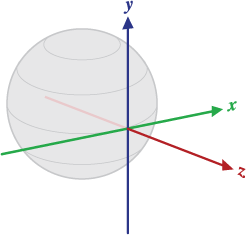
\includegraphics[scale=1]{Gambar/axis-globe.png}
	\caption{Sistem koordinat sensor rotasi vektor terhadap Bumi} 
	\label{fig:axis-globe}
	\end{figure}
	\item values[0]: \(x \sin (\frac{\theta}{2})\)
	\item values[1]: \(y \sin (\frac{\theta}{2})\)
	\item values[2]: \(z \sin (\frac{\theta}{2})\)
	\item values[3]: \(\cos (\frac{\theta}{2})\)
	\item values[4]: Perkiraan akurasi (dalam radians) (-1 jika tidak tersedia) 
\end{itemize}

\end{itemize}
\begin{itemize}
	\item \textbf{Google VR SDK}
\end{itemize}

\label{sec:google_vr_sdk}
Google VR SDK\cite{google_vr_developers} digunakan untuk membantu dalam pembuatan aplikasi Virtual Reality pada \textit{smartphone}. Google VR SDK memberikan beberapa fitur sebagai berikut :
\begin{itemize}
	\item \textbf{Binocular rendering}: Fitur untuk tampilan layar terpisah untuk masing-masing dalam pandangan VR.
	\item \textbf{Spatial audio}: Fitur untuk mengeluarkan suara yang datang dari daerah-daerah tertentu dari dunia VR.
	\item \textbf{Head movement tracking}: Fitur untuk mendapatkan memperbaharui pengelihatan dunia VR yang sesuai dengan gerakan kepala pengguna.
	\item \textbf{Trigger input}: Fitur untuk memberikan input pada dunia VR dengan menekan tombol.
\end{itemize}

Ada beberapa persyaratan untuk menggunakan Google VR SDK, persyaratan tersebut adalah:
\begin{itemize}
	\item Android Studio versi 1.0 atau lebih.
	\item Android SDK versi 23
	\item Gradle versi 23.0.1 atau lebih. Android Studio akan membantu meningkatkan versinya jika versinya terlalu rendah.
	\item Perangkat Android fisik yang menjalankan Android versi 4.4 (KitKat) atau lebih.
\end{itemize}

Dalam membuat aplikasi Google Cardboard VR membutuhkan beberapa API(Application Program Interface) dari Google VR SDK. API-API umum yang akan digunakan adalah sebagai berikut. 
\begin{itemize}
	\item API audio: API untuk mengimplementasikan \textbf{\textit{Spatial Audio}} (Metode untuk menspasialisasikan sumber suara dalam ruang tiga dimensi).
	\item API base: API untuk fondasi dari suatu aplikasi Google VR.
\end{itemize}

\textbf{API Audio}
\label{sec:api_audio}
\cite{google_vr_developers}
API ini membantu developer untuk menspasialisasikan sumber suara dalam tiga dimensi, termasuk jarak dengan tinggi isyarat sumber suara. Pada API ini hanya terdapat satu class utama yaitu \textbf{GvrAudioEngine}. \textbf{GvrAudioEngine} mampu memutarkan suara secara spasial dalam dua cara yang berbeda :
\begin{itemize}
	\item Metode pertama dikenal sebagai \textit{Sound Object rendering}. Metode ini memungkinkan pengguna membuat sumber suara virtual dalam ruang tiga dimensi.
	\item Metode kedua memungkinkan pengguna untuk memutar kembali rekaman \textit{Ambisonic soundfield}. Rekaman \textit{Ambisonic soundfield} adalah file audio \textit{multi-channel} yang telah terspasialisasi.
\end{itemize}
API ini juga dapat memutarkan suara secara \textit{stereo}. Kelas \textbf{GvrAudioEngine} memiliki tiga buah \textit{nested class} yaitu:
\begin{itemize}
	\item GvrAudioEngine.DistanceRolloffModel: Kelas ini mendefinisikan konstanta-konstanta yang merepresentasikan perbedaan jarak dari efek model-model rolloff. 
	\item GvrAudioEngine.MaterialName: Kelas ini mendefinisikan konstanta-konstanta yang merepresentasikan bahan permukaan ruangan untuk disesuaikan dengan efek suara pada suatu ruangan.
	\item GvrAudioEngine.RenderingMode: Kelas ini mendefinisikan konstanta-konstanta untuk menyesuaikan dengan mode rendering. Semakin baik kualitas renderin akan semakin besar penggunaan CPU(Central Processing Unit).
\end{itemize}

\textbf{API Base}
\label{sec:api_base}
\cite{google_vr_developers}
API ini digunakan sebagai fondasi dari suatu aplikasi Google VR. Fitur-fitur Binocular rendering, Head movement tracking, dan Trigger input diimplementasikan pada API ini. Kelas-kelas penting yang ada di API ini adalah AndroidCompat, Eye, GvrActivity, GvrView, HeadTransform, Viewport.
\begin{itemize}
	\item AndroidCompat\\
Kelas ini merupakan kelas utilitas untuk menggunakan fitur VR. Fitur-fitur ini mungkin tidak tersedia pada semua versi android. Kelas ini memiliki method-method sebagai berikut:
\begin{itemize}
	\item setSustainedPerformanceMode(Activity activity, boolean enabled): \\
	Method ini digunakan untuk mengubah window android ke mode performa secara berkelanjutan.
	\item public static void setVrModeEnabled (Activity activity, boolean enabled): \\
	Mengatur pengaturan yang tepat untuk "mode VR" pada suatu Activity. Method ini tidak digunakan karena hanya dapat digunakan pada Android N+.
	\item public static boolean trySetVrModeEnabled (Activity activity, boolean enabled): 
	Method ini kegunaanya sama dengan method \textbf{setVrModeEnabled (Activity activity, boolean enabled)}, namun mengembalikan boolean true jika berhasil dan sebaliknya.
\end{itemize}
	\item Eye\\
Kelas ini mendefinisikan detil perenderan stereoskopik mata. Method penting yang dimiliki kelas ini adalah \textbf{public float[] getEyeView ()}. Method ini mengembalikan matriks yang mentransformasikan camera virtual ke mata. Transformasi yang diberikan termasuk melacak rotasi kepala, perubahan posisi dan perubahan IPD(interpupillary distance).
	\item GvrActivity\\
Kelas ini merupakan Activity dasar yang menyediakan integrasi yang mudah dengan headset Google VR. Kelas ini mengekspos kejadian untuk berinteraksi dengan headset Google VR dan menangani detil-detil yang biasa diperlukan saat membuat suatu Activity untuk perenderan VR. Activity ini membuat layar tetap menyala selama perangkat android bergerak. Jika tidak ada pergerakan dari perangkat android maka layar reguler (\textit{wakeclock}) akan ditampilkan. Pada kelas ini terdapat method \textbf{onCardboardTrigger ()} untuk mendeteksi ketika Cardboard Trigger sedang ditarik dan dilepaskan (Magnet yang berada pada sisi Google Cardboard).
	\item GvrView\\
	Kelas ini merupakan kelas View yang menyediakan perenderan VR. Kelas ini didesain untuk berkerja pada mode layar penuh dengan orientasi \textit{landscape} atau \textit{reverse landscape}. Kelas View ini dapat digunakan dengan mengimplements salah satu Interface perenderan. Interface-interface tersebut adalah:
	\begin{itemize}
		\item GvrView.StereoRenderer: Interface untuk perenderan detil stereoskopik secara abstrak oleh perender.
		\item GvrView.Renderer: Interface untuk mesin yang kompleks yang membutuhkan untuk menangai semua detil perenderan.
	\end{itemize}
Kelas GvrView.Renderer jarang digunakan dan sebaiknya tidak digunakan jika tidak sangat dibutuhkan.
Ketika suatu kelas mengimplement Kelas GvrView.StereoRenderer, kelas tersebut harus mengimplementasikan method-method berikut ini:
\begin{itemize}
	\item \textbf{public void onNewFrame(HeadTransform headTransform)}\\
	method ini terpanggil ketika Framebaru akan digambar. Method ini memungkinkan untuk membedakan antara perenderan pandangan mata dan frame-frame yang berbeda. Setiap operasi per-frame harus tidak spesifik pada satu tampilan saja.
	\item \textbf{public abstract void onDrawEye (Eye eye)}\\
	Method ini meminta untuk menggambar suatu konten dari sudut pandang mata.
	\item \textbf{public abstract void onFinishFrame (Viewport viewport)}\\
	Method ini dipanggil ketika suatu frame telah selesai. Dengan pemanggilan ini, konten frame telah di gambar dan jika koreksi distorsi diaktifkan, koreksi distrosi akan diterapkan. Setiap perendereran pada tahap ini relatif terhadap seluruh permukana, tidak terhadap satu pandangan mata tunggal. 
	\item \textbf{public abstract void onRendererShutdown ()}\\
	Method ini dipanggil ketika thread perender sedang menutup. Melepaskan sumber GL(Graphics Library) dan sedang melakukan penutupan operasi pada thread perender. Dipanggil hanya jika sebelumnya ada pemanggilan method onSurfaceCreated.
	\item \textbf{public abstract void onSurfaceChanged (int width, int height)}\\
	Dipanggil ketika ada perubahan dimensi permukaan. Semua nilai adalah relatif ke ukuran yang dibutuhkan untuk merender sebuah mata.
	\item \textbf{public abstract void onSurfaceCreated (EGLConfig config)}\\
	Method ini dipanggil ketika suatu permukaan dibangun atau dibangun ulang.
\end{itemize}
\item HeadTransform\\
	Method ini mendeskripsikan transformasi kepala secara independen dari setiap parameter mata. Kelas ini digunakan di kelas GvrView.StereoRenderer sebagai parameter pada method \textbf{onNewFrame}. Method-method yang perlu diperhatikan pada kelas ini adalah:
	\begin{itemize}
		\item \textbf{public void getHeadView (float[] headView, int offset)}\\
		Method ini digunakan untuk mendapatkan matriks transformasi dari camera virtual ke kepala. Kepala disini didefinisikan sebagai titik tengah diantara kedua mata. Matriks yang didapatkan akan disimpan pada parameter \textbf{headView}.
		\item \textbf{public void getQuaternion (float[] quaternion, int offset)}\\
		Method ini digunakan untuk mendapatkan kuaternion yang merepresentasikan rotasi kepala.
	\end{itemize}
	\item Viewport\\
	Kelas ini didefinisikan sebagai \textit{viewport}(area pandang) berbentuk persegi.
\end{itemize}



\begin{itemize}
	\item \textbf{Teori Kuaternion}
\end{itemize}
\label{sec:teori_quaternion}
Pada Android SDK \textbf{SensorEvent.values} \cite{android_developers} tipe sensor \textbf{Sensor.TYPE\_ROTATION\_VECTOR}, yaitu tipe sensor yang mendeteksi vektor perputaran pada \textit{smartphone}. Seperti yang sudah di jelaskan pada bagian sebelumnya, tipe sensor ini akan mengembalikan nilai-nilai dari komponen kuaternion. 
Kuaternion\cite{kuipers:1999} adalah objek penggabungan dari suatu skalar dengan suatu vektor, sesuatu yang tidak dapat didefinisikan dalam aljabar linear biasa. Kuaternion ditemukan oleh William Rowan Hamilton dengan memperpanjang notasi dari bilangan kompleks menjadi Kuaternion. \\

\textbf{Struktur Ajabar}\\

Karena Kuaternion merupakan bilangan kompleks yang diperpanjang notasinya, struktur aljabar Kuaternion hampir mirip dengan bilangan kompleks. Untuk mengerti struktur-struktur aljabar kuaternion, diperlukan untuk mengerti  bilangan kompleks terlebih dahulu. Berikut adalah penjelasan singkat tentang bilangan kompleks. \\

Bilangan Kompleks\\

\label{sssec:bilangan_kompleks}
\cite{kuipers:1999}
Bilangan kompleks adalah bilangan yang merupakan gabungan dari bilangan imajiner dengan bilangan riil. Notasi umum dari bilangan kompleks adalah :

\begin{equation}
	a+bi
\label{eq:notasi_umum_bilangan_kompleks}
\end{equation}
Pada notasi \ref{eq:notasi_umum_bilangan_kompleks} bilangan \(a\) dengan \(b\) merupakan bilangan riil, dan \(i\) merupakan bilangan imajiner tertentu yang memiliki sifat \(i^2=-1\). Bilangan kompleks juga dapat beroperasi dengan bilangan kompleks lainnya seperti penjumlahan, perkalian, pengurangan, dan pembagian. Berikut adalah contoh-contoh operasi pada bilangan kompleks \ref{eq:notasi_umum_bilangan_kompleks} dengan bilangan kompleks \(c+di\):
\begin{itemize}
	\item Penjumlahan\\
	\[
	 (a + bi) + (c + di) = (a+c) + i(b+d)
	\]
	\item Perkalian\\
	\[
	 (a + bi)(c + di) = (ac−bd) + (bc+ad)i
	\]
	\item Pengurangan\\
	\[
	 (a + bi) - (c + di) = (a-c) + i(b-d)
	\]
	\item Pembagian\\
	\[
	 \frac{(a + bi)}{(c + di)} = \frac{(ac+bd)}{c^2+d^2} + i \frac{bc-ad}{c^2+d^2}
	\]
\end{itemize}
Pada operasi penjumlahan dan perkalian untuk kedua bilangan kompleks tersebut memiliki hukum assosiatif dan komutatif. Notasi \ref{eq:penjumlahan_hukum} menunjukkan bagaimana  kedua hukum tersebut berlaku pada penjumlahan.
\begin{equation}
	\begin{split}
	(a+ib) + (c+id) = (a+c) + i(b+d)=\\
	(c+id) + (a+ib) = (c+a) + i(d+b)
	\end{split}
\label{eq:penjumlahan_hukum}
\end{equation}

Suatu bilangan dapat dikatakan konjugasi kompleks dari suatu bilangan kompleks jika nilai bilangan riilnya sama, tetapi nilai bilangan imajinernya berlawanan dengan nilai pada bilangan kompleks tersebut. Maka konjugasi kompleks dari bilangan kompleks \ref{eq:notasi_umum_bilangan_kompleks} adalah \(a-bi\). 

Bilangan kompleks ini dapat digunakan untuk rotasi vektor pada bidang dua dimensi. Rotasi ini dapat dilakukan dengan mengalikan suatu vektor dengan bilangan imajiner $i$. Mengalikan suatu vektor dengan bilangan imajiner $i$ akan memutar vektor sebesar $90^{\circ}$ berlawanan arah jarum jam. Mengalikan suatu vektor dengan bilangan imajiner $i^2$ akan memutar vektor sebesar $180^{\circ}$ berlawanan arah jarum jam. Untuk memperjelas perputaran dengan bilangan kompleks diberikan contoh berikut:
Sebuah vektor $v = 3 + i3$ akan diputar $90^{\circ}$ berlawanan arah jarum jam dengan mengalikan vektor tersebut dengan bilangan imajiner $i$. Maka vektor hasil perputarannya($v'$) adalah :
\begin{equation}
	\begin{split}
		v' = &i(3 + i3)\\
		= & i3 + i^2 3\\
		= & i3 + (-1) 3\\
		= & -3 + i3
	\end{split}
\label{eq:rotasi_kompleks}
\end{equation}
\begin{figure}[htbp]
\centering
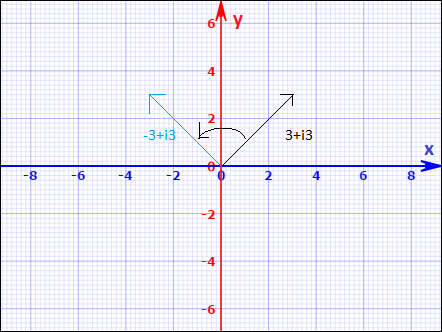
\includegraphics[scale=1]{Gambar/diagram-rotasi-kompleks.png}
\caption{Contoh perputaran dengan bilangan kompleks} 
\label{fig:diagram-rotasi-kompleks}
\end{figure}
Dengan bilangan pada bilangan riil diasumsikan sebagai nilai pada sumbu x dan bilangan yang dikalikan dengan bilangan $i$ diasumsikan pada sumbu y($x + iy$) Seperti yang ditunjukkan pada Gambar \ref{fig:diagram-rotasi-kompleks}. Oleh karena itu rumus perputaran menggunakan bilangan kompleks dapat di rumuskan sebagai berikut: 
\[
	v' = v\times(\cos \theta + i \sin \theta)
\]
dengan $\theta$ adalah besar sudut perputaran. Jika vektor $v = 3 + i3$ diputar $30^{\circ}$ berlawanan arah jarum jam menggunakan konsep diatas, akan menghasilkan vektor berikut:

\begin{equation}
	\begin{split}
		v' = &(3 + i3)(\cos 30^{\circ} + i \sin 30^{\circ})\\
		= & (3 + i3)(\frac{\sqrt{3}}{2} + i \frac{1}{2})\\
		= & \frac{3\sqrt{3}-3}{2} + i\frac{3\sqrt{3}+3}{2}\\
		= & 1.098 + i4.098
	\end{split}
\label{eq:rotasi_kompleks_tiga_puluh_derajat}
\end{equation}

Persamaan \ref{eq:rotasi_kompleks_tiga_puluh_derajat} dapat divisualisasikan pada Gambar \ref{fig:diagram-rotasi-kompleks1}.

\begin{figure}[htbp]
\centering
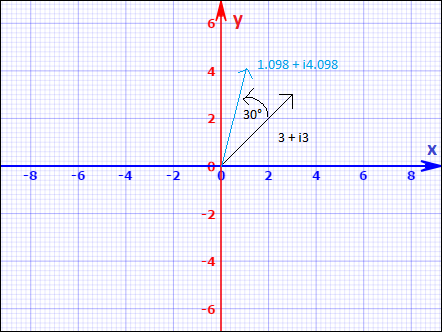
\includegraphics[scale=1]{Gambar/diagram-rotasi-kompleks1.png}
\caption{Contoh perputaran tiga puluh derajat dengan bilangan kompleks} 
\label{fig:diagram-rotasi-kompleks1}
\end{figure}

		\item Merancang dan Membuat aplikasi untuk menampilkan grafik sensor-sensor pada smartphone Android.\\
		{\bf status :} Ada sejak rencana kerja skripsi.\\
		{\bf hasil :}
		
Analisis grafik data sensor-sensor pada Android dilakukan dengan membuat suatu aplikasi perekam sensor-sensor yang ada pada \textit{smartphone} Android terlebih dahulu. Aplikasi ini akan merekam nilai-nilai yang dihasilkan dari sebagian sensor-sensor pada android setiap ada perubahan. Pada skripsi ini, nilai sensor-sensor yang dibutuhkan adalah sensor \textit{accelerometer}, \textit{gyroscope}, \textit{rotation vector}, dan \textit{geomagnetic rotation}. Aplikasi menyimpan nilai sensor-sensor menggunakan format CSV \textit{(Comma Separated Values)}. Format CSV adalah format penulisan suatu file dengan menggunakan koma (,) sebagai pemisah antara nilai-nilai pada file. Dari data yang diperoleh oleh apliasi tersebut dibuatkan grafiknya menggunakan aplikasi Microsoft Excel. Penjelasan dari setiap grafik akan dijelaskan pada bagian analisi grafik dari sensor-sensor pada \textit{smartphone} ketika mengangguk dan menggeleng.  	

		\item Menganalisis aplikasi-aplikasi sejenis.\\
		{\bf status :} Ada sejak rencana kerja skripsi.\\
		{\bf hasil :}



Aplikasi sejenis pada perangkat \textit{Virtual Reality} Google Cardboard hanyalah ada satu aplikasi saja. Aplikasi tersebut adalah aplikasi InMind VR. Aplikasi sejenis pada perangkat \textit{Virtual Reality} Oculust Rift adalah Trial of the Rift Drifter dengan Asunder yang di kembangkan oleh AldinDynamics \cite{aldin_dynamics}. Aplikasi sejenis pada \textit{Virtual Reality} Oculust Rift tidak dapat dianalisis karena penulis tidak memiliki perangkat Oculust Rift. 
\textbf{Analisis InMind VR}

InMind VR merupakan permainan \textit{Virtual Reality} yang seakan-akan pengguna berada dalam sel-sel otak seorang manusia. Permainan ini dimainkan dengan mengarahkan arah pandang kepala ke arah sel-sel neuron yang dapat menyebabkan gangguan mental (Gambar \ref{fig:screenshot_inmind_task}). Akan ada 50 sel neuron yang dapat menyebabkan gangguan mental. Sel-sel yang dapat menyebabkan gangguan mental adalah sel-sel yang berwarna merah seperti pada Gambar \ref{fig:screenshot_inmind_gameplay}.

\begin{figure}[H]
\centering
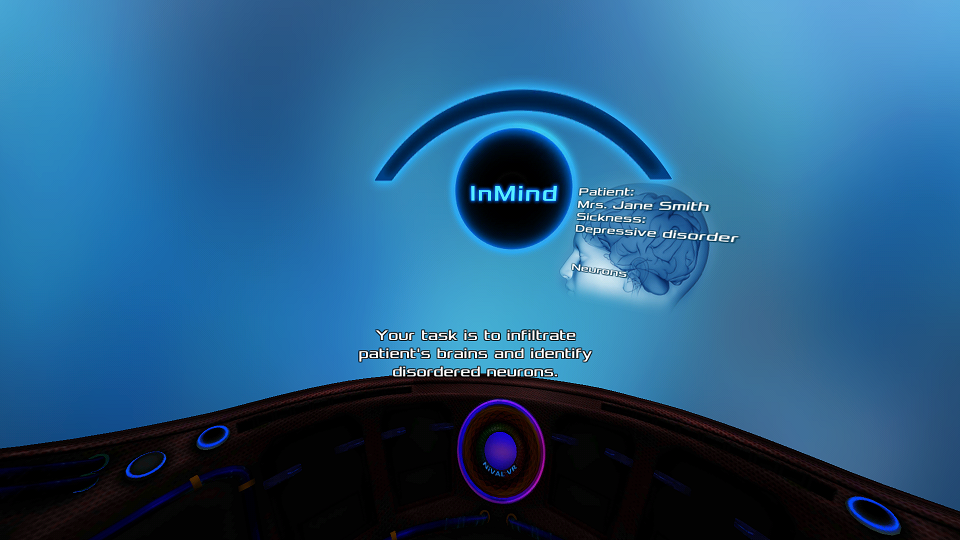
\includegraphics[scale=0.6]{Gambar/screenshot-inmind-task.png}
\caption{\textit{Screenshot} task yang diberikan aplikasi InMind VR.}
\label{fig:screenshot_inmind_task}
\end{figure}

Pada permulaan permainan pengguna diberi pertanyaan apakah pengguna sudah siap untuk melakukan permainan tersebut seperti yang ditunjukkan pada Gambar \ref{fig:screenshot_inmind_nod}.

\begin{figure}[H]
\centering
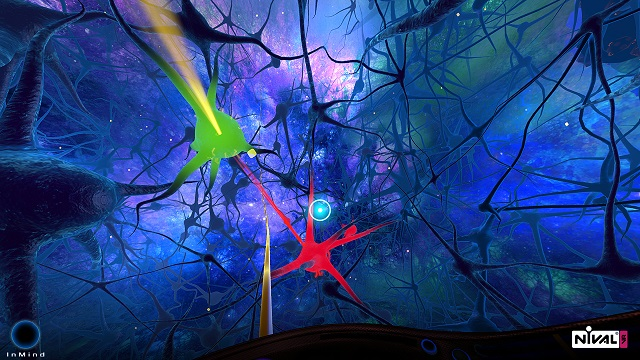
\includegraphics[scale=0.7]{Gambar/screenshot-inmind-gameplay.jpg}
\caption{\textit{Screenshot} aplikasi InMind VR ketika permainan berlangsung.}
\label{fig:screenshot_inmind_gameplay}
\end{figure}

Analisis dilakukan dengan cara mengetes aplikasi ini dengan mengangguk dan menggeleng yang spesifik. Mengangguk dilakukan dengan cara-cara berikut:
\begin{enumerate}
	\item Mengangguk secara pelan.
	\item Mengangguk yang diawali dengan gerakan ke atas.
	\item Melihat kebawah saja tanpa membalikkan kepala ke posisi semula.
	\item Tidak menggerakkan kepala sama sekali.
\end{enumerate}

Dari keempat percobaan mengangguk yang dilakukan, hanya percobaan pertama dengan percobaan ketiga yang terdeteksi mengangguk. Aplikasi ini dapat disimpulkan dengan hanya menggerakkan kepala kebawah saja sudah dapat dianggap mengangguk oleh aplikasi ini. Pada percobaan kedua dan keempat terjadi keganjilan dari pendeteksian anggukkan. Pada percobaan kedua dan keempat aplikasi tetap akan melanjutkan permainan setelah beberapa detik berlalu. Sel-sel yang dapat menyebabkan gangguan mental adalah sel-sel yang berwarna merah seperti pada Gambar \ref{fig:screenshot_inmind_gameplay}. 

Ketika dilakukan percobaan menggeleng, tidak ada respon apapun dari aplikasi ini. Aplikasi ini akan tetap melanjutkan ke permainan setelah beberapa detik telah berlalu. Hal tersebut menyimpulkan bahwa aplikasi ini tidak dapat mendeteksi gerakan menggeleng. Oleh karena itu hal yang dilakukan oleh aplikasi ini hanyalah melihat apakah pengguna sudah melihat kebawah atau belum saja.

\begin{figure}[H]
\centering
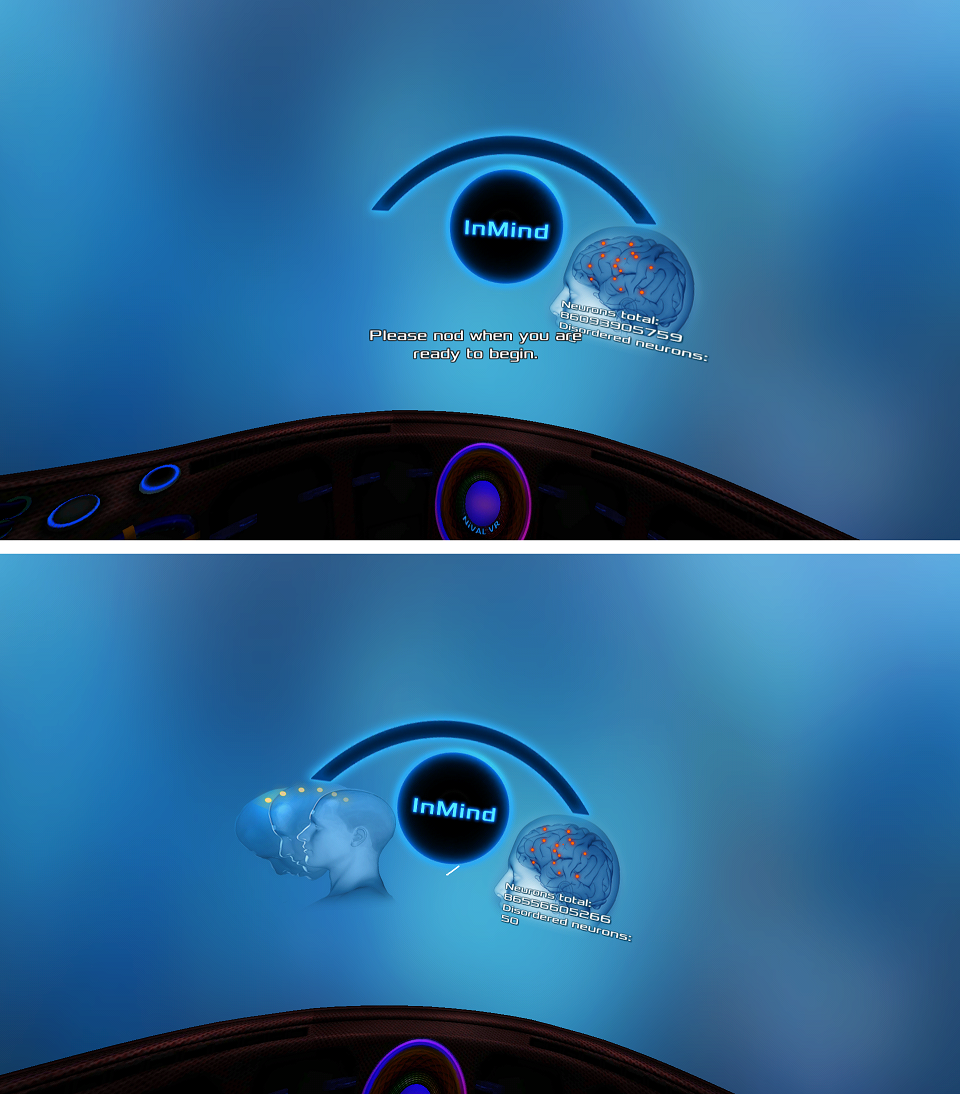
\includegraphics[scale=0.6]{Gambar/screenshot-inmind-nod.png}
\caption{\textit{Screenshot} aplikasi InMind VR ketika meminta pengguna untuk mengangguk jika telah siap.}
\label{fig:screenshot_inmind_nod}
\end{figure}

		\item Merekam dan menganalisis grafik dari sensor-sensor pada \textit{smartphone} ketika mengangguk dan menggeleng.\\
		{\bf status :} Ada sejak rencana kerja skripsi.\\
		{\bf hasil :}
		
		
\begin{itemize}
	\item \textbf{Perekaman Data Sensor}
\end{itemize}
\label{sec:perekaman_data_sensor}

Pada analisis ini akan dilakukan perekaman mengganguk dan menggeleng dengan sensor-sensor pada Android. Perekaman-perekaman ini akan dilakukan pada tiga kondisi muka pengguna. Kondisi muka yang pertama adalah kondisi muka pengguna ketika menghadap ke depan, digambarkan dengan Gambar \ref{fig:posisi-muka} bagian (a). Kondisi muka yang kedua adalah kondisi muka pengguna keita menghadap ke atas sekitar $45^{\circ}$ dari pandangan muka menghadap ke atas digambarkan dengan Gambar \ref{fig:posisi-muka} bagian (b). Kondisi muka yang ketiga adalah kondisi muka ketika menghadap serong ke kiri atas digambarkan dengan Gambar \ref{fig:posisi-muka} bagian (c). Anggukan yang dilakukan oleh pengguna hanya sebanyak satu kali mengangguk ke bawah saja. Sedangkan dalam menggeleng akan bergerak ke kiri terlebih dahulu dan ke kanan setelahnya dan diakhiri pada posisi muka kembali ke posisi awal.

\begin{figure}[htbp]
\centering
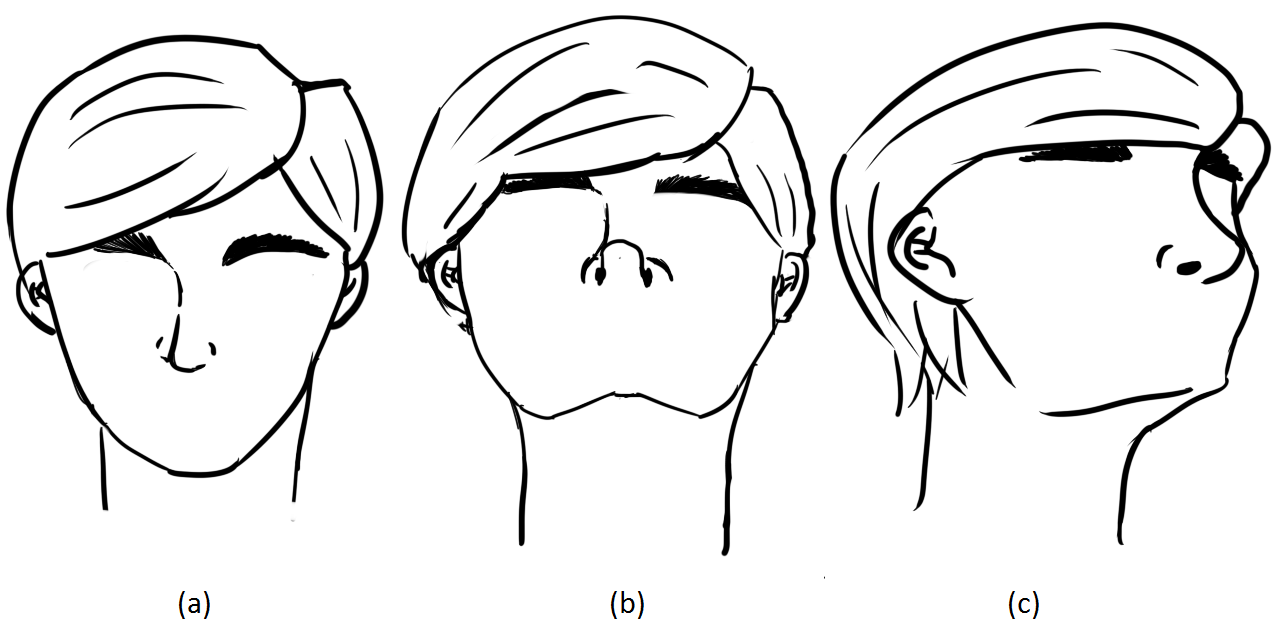
\includegraphics[scale=0.4]{Gambar/posisi-muka.png}
\caption{Gambar untuk mendeskripsikan posisi dari muka sebelum melakukan gerakan menggeleng atau mengangguk. Gambar (a) adalah kondisi muka ketika sedang menghadap ke depan. Gambar (b) adalah kondisi muka ketika sedang menghadap ke atas. Gambar(c) adalah kondisi muka ketika sedang menghadap ke serong kiri atas.}
\label{fig:posisi-muka}
\end{figure}

Grafik-grafik yang akan ditunjukkan pada bab ini akan memiliki beberapa karakteristik. Sumbu y pada grafik yang akan ditunjukkan akan merepresentasikan besar nilainya, Sedangkan sumbu x akan merepresentasikan waktunya. Grafik yang ditunjukkan akan memiliki beberapa nilai, tergantung dari jumlah nilai yang dikembalikan untuk setiap sensornya. Contohnya pada sensor \textit{accelerometer} yang memiliki tiga jenis nilai, sehingga pada grafik akan terbentuk tiga buah garis nilai. Aplikasi akan merekam beberapa sensor secara langsung ketika pengguna mengangguk atau menggeleng, sehingga nilai wakunya akan sama untuk kondisi muka yang sama walaupun sensornya berbeda.

Analisis grafik data sensor-sensor pada Android dilakukan dengan membuat suatu aplikasi perekam sensor-sensor yang ada pada \textit{smartphone} Android terlebih dahulu. Aplikasi ini akan merekam nilai-nilai yang dihasilkan dari sebagian sensor-sensor pada android setiap ada perubahan. Pada skripsi ini, nilai sensor-sensor yang dibutuhkan adalah sensor \textit{accelerometer}, \textit{gyroscope}, \textit{rotation vector}, dan \textit{geomagnetic rotation}. Aplikasi menyimpan nilai sensor-sensor menggunakan format CSV \textit{(Comma Separated Values)}. Dari data yang diperoleh oleh apliasi tersebut dibuatkan grafiknya menggunakan aplikasi Microsoft Excel. Penjelasan dari setiap grafik akan dijelaskan pada bagian berikut.\\

\textbf{Perekaman Grafik Sensor \textit{Accelerometer}}\\

\label{sec:analisis_grafik_sensor_accelerometer}
Seperti yang sudah dijelaskan pada bab sebelumnya, sensor \textit{accelerometer} akan mendeteksi seluruh percepatan yang terjadi pada perangkat Android. Perekaman ini perangkat android akan diletakkan di depan muka pengguna, sehingga percepatan yang mempengaruhi perangkat Android hanya percepatan gravitasi dengan percepatan yang dilakukan oleh gerakan kepala pengguna. 

\begin{figure}[htbp]
\centering
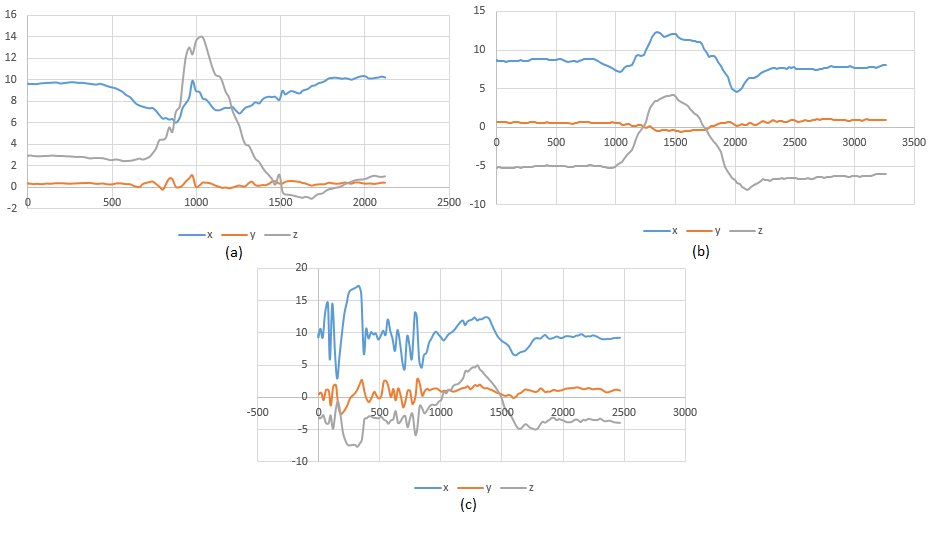
\includegraphics[scale=0.6]{Gambar/grafik-sensor-accelerometer-mengangguk.png}
\caption{Grafik nilai kuaternion dari sensor \textit{accelerometer} ketika pengguna mengangguk dengan posisi muka awal (a) menghadap ke depan, (b) menghadap ke atas, (c) menghadap ke kiri atas.} 
\label{fig:grafik-sensor-accelerometer-mengangguk}
\end{figure}

Gambar \ref{fig:grafik-sensor-accelerometer-mengangguk} merupakan grafik-grafik yang terbentuk dari nilai yang di terima oleh sensor \textit{accelerometer} ketika pengguna sedang mengangguk. Pada Gambar \ref{fig:grafik-sensor-accelerometer-mengangguk} grafik (a) terlihat nilai z menaik dan nilai x menurun ketika sedang mengangguk. Tetapi nilai x kembali menaik ketika nilai z sudah hampir mencapai nilai tertinggi. Sedangkan nilai y terlihat cukup konstan di sekitar angka 0. Pada grafik (b) terlihat nilai x dengan y memiliki pola yang serupa ketika mengangguk. Kedua nilai menaik ketika pengguna sedang mengangguk. Nilai x bermulai dari nilai sekitar sebesar 9 sedangkan nilai z bernilai sekitar sebesar -5. Sama seperti pada grafik (a) nilai y terlihat konstan di sekitar angka 0. Selanjutnya grafik (c) pada Gambar \ref{fig:grafik-sensor-accelerometer-mengangguk} merupakan grafik yang terbentuk dari nilai yang diterima oleh sensor \textit{accelerometer} ketika pengguna mengangguk dan sedang menghadap ke kiri atas. Grafik pada bagian ini sangat tidak beraturan. Pada Grafik ini sulit untuk membedakan kondisi kapan pengguna sedang mengangguk. Goncangan yang terjadi terhadap \textit{smartphone}, seperti munculnya notifikasi mungkin dapat menyebabkan hal ini. Namun pada waktu mencapai 1000 milidetik terlihat cukup stabil. Pada grafik (c) di Gambar \ref{fig:grafik-sensor-accelerometer-mengangguk} juga menunjukkan bahwa nilai x dengan z memiliki pola yang sama hingga akhir, dan nilai y konstan di sekitar angka 0. Hasil nilai tersebut serupa dengan kasus ketika menghadap ke atas. 


\begin{figure}[htbp]
\centering
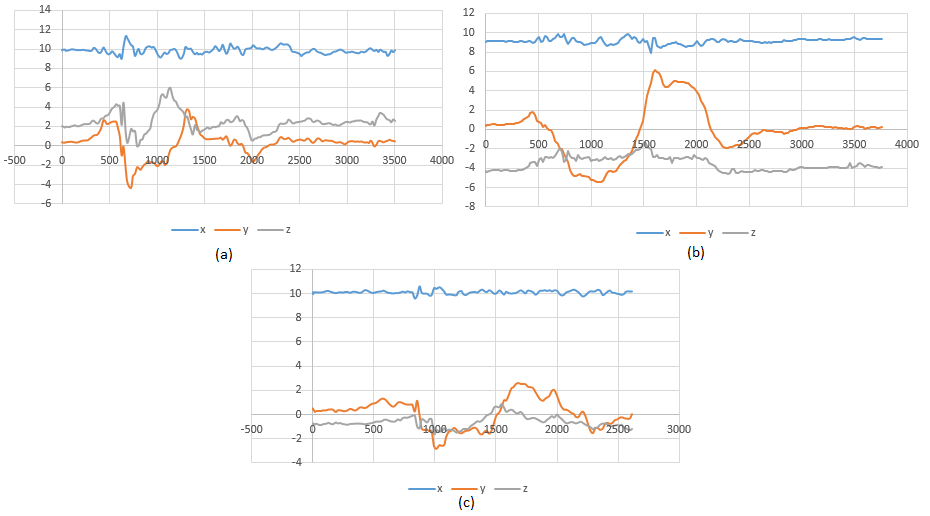
\includegraphics[scale=0.6]{Gambar/grafik-sensor-accelerometer-menggeleng.png}
\caption{Grafik nilai kuaternion dari sensor \textit{accelerometer} ketika pengguna menggeleng dengan posisi muka awal (a) menghadap ke depan, (b) menghadap ke atas, (c) menghadap ke kiri atas.} 
\label{fig:grafik-sensor-accelerometer-menggeleng}
\end{figure}

Gambar \ref{fig:grafik-sensor-accelerometer-menggeleng} merupakan grafik yang terbentuk dari nilai yang diterima oleh sensor \textit{accelerometer} ketika pengguna menggeleng. Pada grafik (a), nilai x konstan di sekitar angka 10. Nilai y dengan z pada grafik (a) menaik dan menurun ketika pengguna menggelengkan kepala. Pada grafik (b) nilai x terlihat konstan di sekitar nilai 10 dan nilai z sedikit tidak beraturan di sekitar nilai -4 hingga -2. Nilai y mengalami kenaikan dan penurunan saat menggeleng. Pada grafik (c) di Gambar \ref{fig:grafik-sensor-accelerometer-menggeleng} nilai x konstan di sekitar nilai 10. Nilai y menaik dan menurun, tetapi tidak beraturan. Nilai pada z juga mengalami sedikit kenaikan dan penurunan. Pada grafik (b) dengan (c) nilai z mengalami perubahan yang tidak beraturan dan puncak tertinggi dengan puncak terendahnya tidak terlalu berbeda jauh dengan nilai awalnya.

Dari keenam grafik tersebut terlihat bahwa nilai yang terpengaruh ketika pengguna sedang mengangguk adalah nilai x dengan z. Nilai y tidak berpengaruh karena nilai y cenderung konstan. Nilai yang terpengaruh ketika pengguna sedang menggeleng adalah nilai y. Nilai x terlihat konstan pada setiap grafik, tetapi nilai z mengalami sedikit pergerakan ketika pengguna sedang mengangguk sehingga tidak dapat dipastikan bahwa nilai z terpengaruhi gerakan menggeleng. \\

\textbf{Perekaman Grafik Sensor \textit{Gyroscope}}\\

\label{sec:analisis_grafik_sensor_gyroscope}
Perekaman menggunakan sensor \textit{gyroscope} akan mendapatkan percepatan angular yang terjadi setiap waktunya. Berbeda dengan sensor \textit{accelerometer} yang dapat terpengaruhi oleh lingkungan sekitar seperti gravitasi dan percepatan lainnya, sensor ini hanya akan merekam perputaran yang terjadi pada perangkat saja. Hal ini sangat menguntungkan dalam mendeteksi suatu gerakan karena tidak harus memperdulikan kasus dari pengaruh luar. 


\begin{figure}[htbp]
\centering
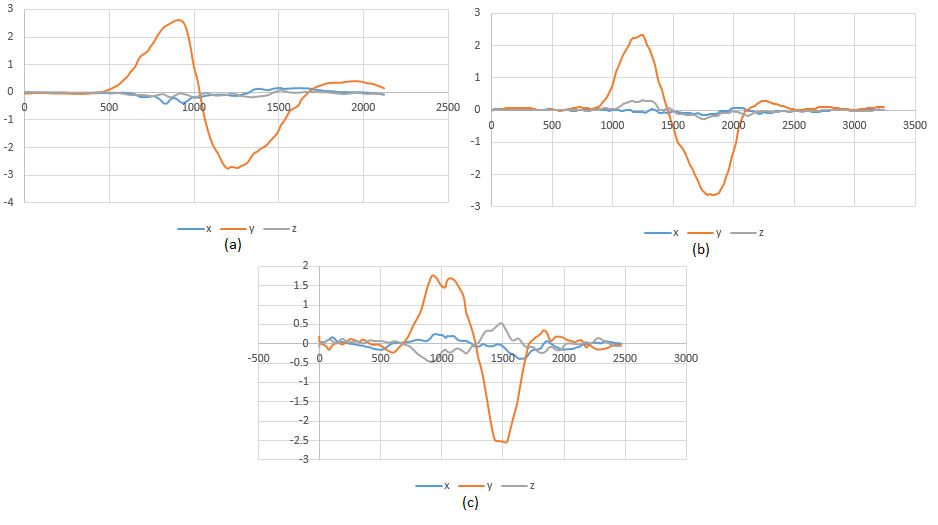
\includegraphics[scale=0.6]{Gambar/grafik-sensor-gyroscope-mengangguk.png}
\caption{Gambar grafik nilai sensor \textit{gyroscope} ketika pengguna mengangguk dengan posisi muka awal (a) menghadap ke depan, (b) menghadap ke atas, (c) menghadap ke kiri atas.}
\label{fig:grafik-sensor-gyroscope-mengangguk}
\end{figure}
Gambar \ref{fig:grafik-sensor-gyroscope-mengangguk} menunjukkan nilai-nilai sensor \textit{gyroscope} ketika pengguna sedang mengangguk. Grafik (a) membentuk sebuah bukit dan lembah pada nilai y. Bukit yang terjadi disini menunjukkan ketika pengguna menggerakan kepalanya kebawah, dan ketika kepala pengguna kembali ke posisi semula percepatan angularnya berbalik arah sehingga menimbulkan lembah. Nilai x dengan z cenderung bernilai 0. Grafik (b) mirip seperti grafik pada Gambar \ref{fig:grafik-sensor-gyroscope-mengangguk}. Begitu pula pada grafik (c) yang memiliki pola yang serupa dengan yang grafik-grafik sebelumnya.

\begin{figure}[htbp]
\centering
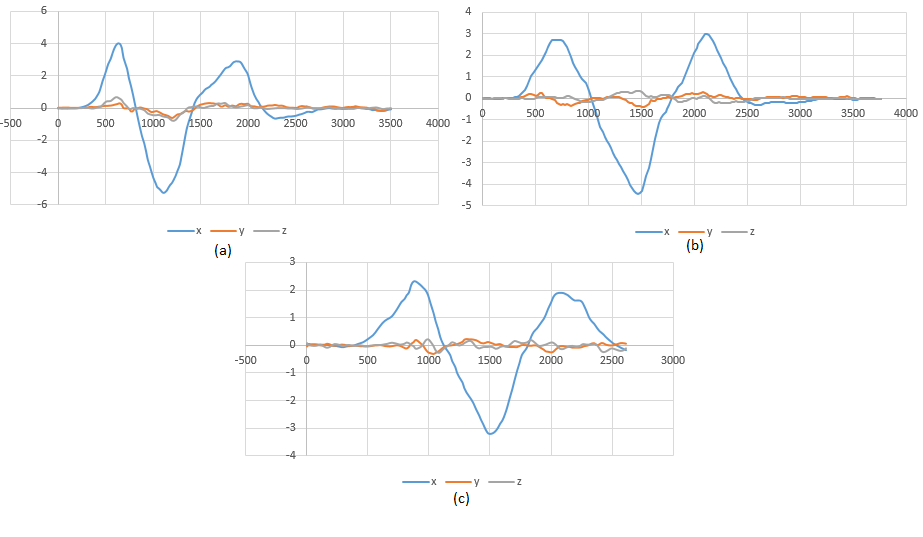
\includegraphics[scale=0.6]{Gambar/grafik-sensor-gyroscope-menggeleng.png}
\caption{Gambar grafik nilai sensor \textit{gyroscope} ketika pengguna menggeleng dengan posisi muka awal (a) menghadap ke depan, (b) menghadap ke atas, (c) menghadap ke kiri atas.} 
\label{fig:grafik-sensor-gyroscope-menggeleng}
\end{figure}

Gambar \ref{fig:grafik-sensor-gyroscope-menggeleng} menunjukkan nilai-nilai sensor \textit{gyroscope} ketika pengguna sedang menggeleng. Pada grafik (a) nilai yang mengalami kenaikan dan penurunan adalah nilai x dan nilai-nilai lainnya cenderung berada pada nilai 0. Nilai x membentuk 2 buah bukit dan 1 buah lembah. Bukit pertama terjadi ketika pengguna menggerakan kepalanya ke kiri. Lembah pertama terjadi ketika pengguna menggerakan kepalanya ke kanan. Bukit kedua terjadi ketika pengguna menggerakan kepalanya kembali ke posisi semula. Pada grafik (b) dengan grafik (c) menunjukkan pola grafik yang serupa dengan grafik pada Gambar (a).

Dari hasil-hasil tersebut dapat disimpulkan bahwa arah pandang pengguna tidak mempengaruhi sensor \textit{gyroscope} dalam mendeteksi gerakan kepala. Nilai-nilai yang dikembalikan oleh sensor \textit{gyroscope} memiliki  pola grafik yang jauh lebih rapih dibandingkan grafik-grafik yang dihasilkan oleh sensor \textit{accelerometer}. Selain itu sensor gyroscope hanya menggunakan 1 jenis nilai yang dipengaruhi oleh pergerakan kepala, sedangkan accelerometer ada 2 jenis nilai yang di pengaruhi gerakan kepala pada saat mengangguk. Oleh karena itu sensor gryoscope lebih baik dalam mendeteksi gerakan yang terjadi pada perangkat android.\\

\textbf{Perekaman Grafik Sensor \textit{Rotation Vector}}\\

\label{sec:analisis_grafik_sensor_rotation_vector}

Perekaman menggunakan sensor \textit{rotation vector} akan mendapatkan sebuah kuaternion yang merepresentasikan perputaran yang terjadi pada perangkat Android. Perputaran ini akan dideskripsikan dengan suatu vektor sebagai sumbu putarnya dan sudut perputarannya. Berbeda dengan sensor \textit{gyroscope} yang merekam kecepatan perputaran yang terjadi pada suatu waktu, sensor \textit{rotation vector} akan mengembalikan nilai kuaternion untuk mendefinisikan suatu kondisi putaran pada saat itu. 

\begin{figure}[htbp]
\centering
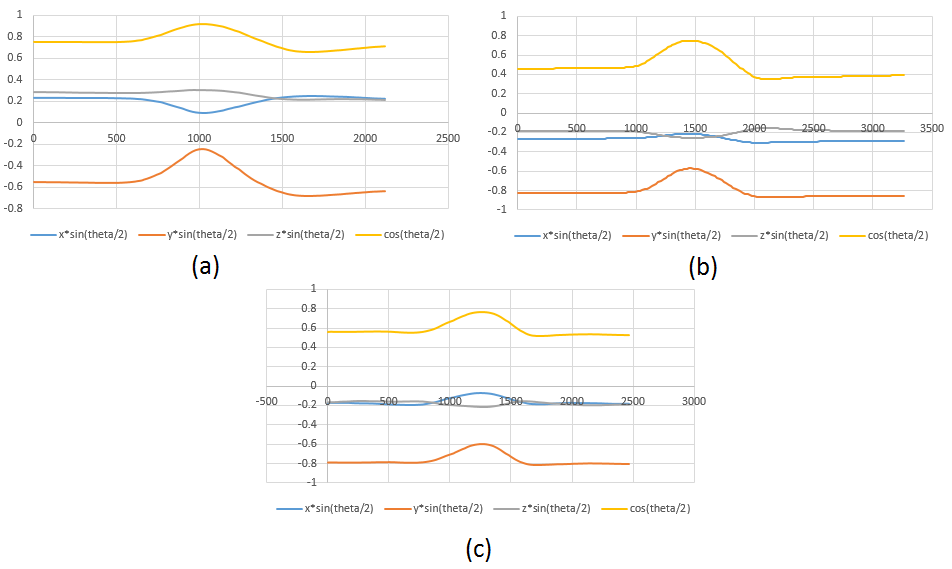
\includegraphics[scale=0.6]{Gambar/grafik-sensor-rot-vector-mengangguk.png}
\caption{Grafik nilai kuaternion dari sensor \textit{rotation vector} ketika pengguna mengangguk dengan posisi muka awal (a) menghadap ke depan, (b) menghadap ke atas, (c) menghadap ke kiri atas.} 
\label{fig:grafik-sensor-rot-vector-mengangguk}
\end{figure}

Gambar \ref{fig:grafik-sensor-rot-vector-mengangguk} menunjukkan nilai-nilai sensor \textit{rotation vector} ketika pengguna sedang mengangguk. Pada grafik (a) terbentuk sebuah bukit pada garis berwarna jingga dengan kuning, dan lembah pada garis berwarna biru. Garis yang berwarna abu cenderung stabil di angka 0.3. Grafik (b) menunjukkan pola yang mirip pada bagian (a) namun berbeda nilainya saja. Pada grafik (a) garis berwarna kuning dimulai pada angka sekitar 0.7, sedangkan pada grafik (b) garis berwarna jingga dimulai pada angka sekitar 0.4. Garis biru pada grafik ini tidak membentuk sebuat lembah seperti  pada grafik pada grafik (a). Garis berwarna abu cenderung konstan pada nilai -0.2, sedangkan pada grafik (a) cenderung konstan di sekitar 0.3. Garis berwarna jingga memiliki pola yang sama dengan garis berwarna kuning, hanya berbeda pada nilainya saja. Seperti pada grafik-grafik sebelumnya, grafik (c) ini memiliki pola yang sama dengan grafik lainnya. Grafik ini juga hanya nilainya saja yang berbeda dengan grafik lainnya. Kemiripan pola ini memungkinkan mempermudah pendeteksian gerakan kepala. 

\begin{figure}[htbp]
\centering
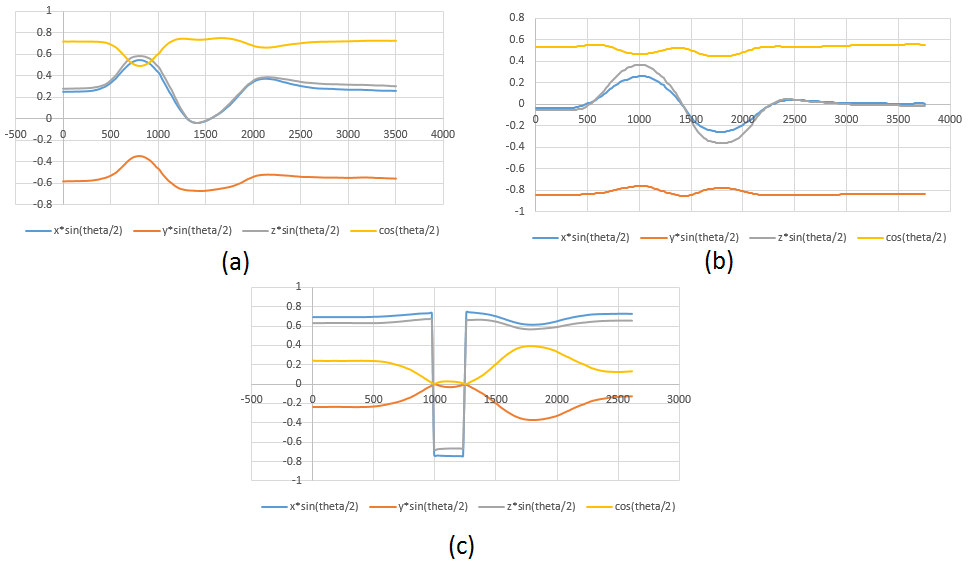
\includegraphics[scale=0.6]{Gambar/grafik-sensor-rot-vector-menggeleng.png}
\caption{Grafik nilai kuaternion dari sensor \textit{rotation vector} ketika pengguna menggeleng dengan posisi muka awal (a) menghadap ke depan, (b) menghadap ke atas, (c) menghadap ke kiri atas.} 
\label{fig:grafik-sensor-rot-vector-menggeleng}
\end{figure}

Gambar \ref{fig:grafik-sensor-rot-vector-menggeleng} menunjukkan nilai-nilai sensor \textit{rotation vector} ketika pengguna sedang menggeleng. Pada grafik (a) terbentuk sebuh bukit yang diikuti dengan lembah pada garis berwarna biru dengan abu-abu. Garis berwarna kuning membentuk suatu lembah yang setelahnya cenderung konstan. Berbeda pada garis kuning yang membentuk bukit kemudian setelahnya cenderung konstan. Grafik (b) memiliki kemiripan dengan grafik (a), garis biru dengan garis abu-abu memiliki pola yang sama yaitu membentuk bukit dengan lembah ketika pengguna menggelengkan kepala. Garis kuning dengan jingga cenderung konstan, berbeda dengan grafik (a) yang membentuk bukit atau lembah. Pada grafik (c) garis-garis membentuk suatu pola yang tidak normal. Garis kuning membentuk sebuah lembah, tetapi membentuk suatu bukit kecil ketika nilainya mencapai nilai 0 pada milidetik ke 1000. Garis jingga memiliki pola yang berlawanan dengan garis kuning. Pada saat garis kuning dengan garis jingga mencapai angka 0 perubahan drastis pun terjadi pada garis biru dengan abu-abu. Pada milidetik ke 1000 garis biru dengan abu mengalami perubahan nilai yang sangat drastis. Kedua nilai tersebut berubah dari nilai yang berkisar diantara 0.6 sampai 0.7 menjadi berkisar diantara -0.7 sampai -0.8. Kasus ini tidak berarti sensor sedang mengalami kegagalan akurasi (\textit{accuracy fail}), tetapi memang seperti itulah karakteristik dari perputaran menggunakan kuaternion pada android. Perputaran yang terjadi pada batas mendekati sebelum terjadinya dengan setelah perubahan nilai yang drastis memiliki hasil perputaran yang sama. Hal ini disebabkan karena melakukan perputaran dengan vektor sebagai sumbu dapat memiliki 2 buah nilai yang sejenis. Dua buah nilai tersebut akan menghasilkan perputaran yang sama ketika arah vektor dengan arah putarnya di balikkan seperti yang ditunjukkan pada Gambar \ref{fig:penjelasan-perputaran-quaternion-android-sensor}. Sepertinya pada sistem android nilai $\cos (theta/2)$ didesain agar tidak bernilai negatif, sehingga nilai-nilai yang lainnya akan mengalami perubahan nilai yang drastis ketika nilai $\cos (theta/2)$ mencapai angka 0.

\begin{figure}[htbp]
\centering
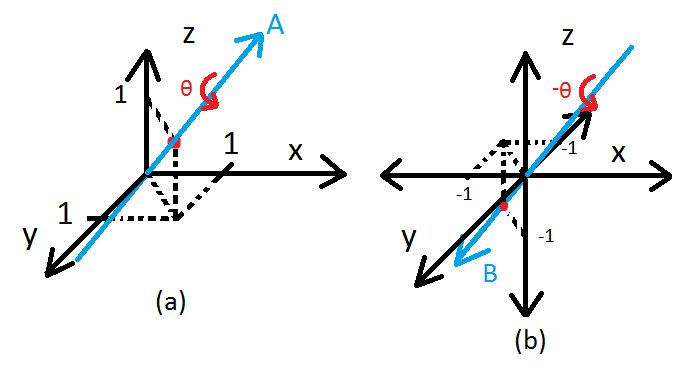
\includegraphics[scale=0.6]{Gambar/penjelasan-perputaran-quaternion-android-sensor.png}
\caption{Dua buah rotasi yang identik dengan nilai kuaternion yang berbeda.} 
\label{fig:penjelasan-perputaran-quaternion-android-sensor}
\end{figure}


\begin{itemize}
	\item Analisis Data Sensor untuk Mendeteksi Gerakan Kepala
\end{itemize}


Dari ketiga hasil pecobaan pada sensor-sensor pada bab \ref{sec:perekaman_data_sensor} dapat disimpulkan bahwa sensor \textit{gyroscope} adalah sensor yang terbaik untuk mendeteksi gerakan kepala. Data dari sensor \textit{accelerometer} akan susah untuk digunakan dalam mendeteksi gerakan kepala karena terganggu dengan aktivitas-aktivitas diluar gerakan pengguna yang juga ikut terekam oleh sensor \textit{accelerometer}. Data dari sensor \textit{rotation vector} juga akan lebih rumit dibandingkan sensor \textit{gyroscope}. Hal ini karena perputaran yang di rekam oleh sensor \textit{rotation vector} merekam kondisi putar pada suatu saat. Hasil rekaman ini akan mempersulit pada saat pendeteksian gerakan kepala karena harus melakukan proses untuk menghitung kecepatan kepala bergerak, agar dapat membedakan gerakan mengangguk atau menggeleng atau sekedar menoleh biasa. 
Dalam mendeteksi gerakan mengangguk dengan menggeleng banyak batas-batas yang perlu diperhatikan. Batas-batas tersebut untuk mengetahui apakah pengguna benar-benar mengangguk atau menggeleng atau sekedar menoleh biasa. Batas-batas yang perlu diperhatikan adalah:

\begin{itemize}
	\item Kecepatan pengguna menoleh.
	\item Jarak waktu pada saat pengguna melakukan melawan arah gerakan.
	\item Simpangan terbesar kepala saat mengangguk atau menggeleng.
\end{itemize}

Kecepatan pengguna menjadi batas karena gerakan kepala yang kecepatannya cenderung pelan biasanya bukan merupakan gerakan mengangguk ataupun menggeleng. Kecepatan ini dapat langsung diperoleh menggunakan sensor \textit{gyroscope}. Kecepatan yang dibutuhkan adalah kecepatan perputaran maksimum yang dilakukan oleh pengguna. Kecepatan maksimum dapat diperoleh dengan mengambil nilai puncak tertinggi dengan terendah. Jika nilai puncaknya mencapai kecepatan tertentu, gerakan tersebut dapat diperkirakan merupakan gerakan mengangguk ataupun menggeleng.

Gerakan menggeleng atau mengangguk biasanya memiliki selang waktu yang sangat sempit, karena pengguna biasanya langsung melawan arah secara langsung ketika sedang mengangguk ataupun menggeleng. Nilai ini dapat diperoleh dengan menghitung jarak antara bukit dengan lembah yang terbentuk pada grafik seperti yang dijelaskan pada Gambar \ref{fig:grafik-penjelasan-jarak-waktu-melawan-gerakan}. Idealnya gerakan menggeleng tidak memiliki rentang waktu ini, namun mungkin sebagian orang masih menghasilkan rentang waktu yang cukup sedikit. Oleh karena itu mungkin batas waktu yang ditentukan di sini adalah sekitar 100 milidetik. Jika rentang waktunya melebihi batas waktu tersebut, maka gerakan tersebut mungkin bukan merupakan gerakan mengangguk ataupun gerakan menggeleng. 

\begin{figure}[htbp]
\centering
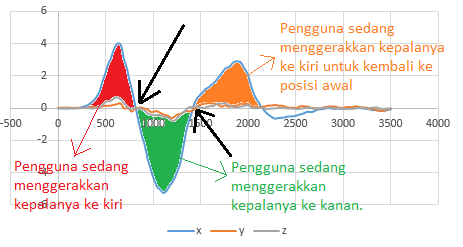
\includegraphics[scale=0.6]{Gambar/grafik-penjelasan-jarak-waktu-melawan-gerakan.png}
\caption{Deskripsi grafik pada saat pengguna menggeleng. Yang ditunjuk oleh panah berwarna hitam adalah selang waktu yang terjadi saat pengguna melawan arah gerakan kepala.} 
\label{fig:grafik-penjelasan-jarak-waktu-melawan-gerakan}
\end{figure}

Simpangan terbesar ini juga penting untuk dijadikan batasan-batasan dalam mendeteksi gerakan mengangguk ataupun menggeleng. Simpangan kepala yang sangat kecil dapat diragukan untuk dianggap sebagai gerakan mengangguk atau menggeleng. Simpangan ini dapat diperoleh dengan menghitung luas yang dibentuk dari bukit atau lembah yang terbentuk pada grafik. Contoh pada Gambar \ref{fig:grafik-penjelasan-jarak-waktu-melawan-gerakan} simpangan terbesar yang terjadi ketika pengguna menggerakkan kepalanya pertama kali ke kiri adalah luas pada bidang yang diarsir merah. Simpangan terbesar yang terjadi ketika pengguna menggerakaan kepalanya ke kanan adalah luas bidang yang diarsir berwarna hijau dikurangi dengan luas pada bidang yang diarsir merah. Pengurangan ini dilakukan karena luas bidang yang diarsir berwarna hijau merupakan simpangan yang terjadi setelah kepala sudah menghadap ke kiri. Begitu pula dengan luas bidang yang diarsir berwarna jingga yang akan dikurangi dengan hasil pengurangan luas sebelumnya.

		\item Menganalisis metode pendeteksi gerakan kepala.\\
		{\bf status :} Ada sejak rencana kerja skripsi.\\
		{\bf hasil :}
		

Seperti yang sudah dijelaskan pada bagian Android Sensor Framework, data akan didapatkan setiap ada perubahan nilai pada sensor dengan rentang waktu tertentu, bergantung dengan konfigurasinya. Pendeteksian ini membutuhkan data yang \textit{real-time}, sehingga akan lebih baik jika menggunakan konfigurasi kecepatan pengambilan data setiap 20.000 mikrodetik. Penggunaan konfigurasi dengan kecepatan 0.000 mikrodetik tidak terlalu baik, karena akan menggunakan kemampuan processor yang sangat tinggi.

\textbf{Algoritma Mendeteksi Gerakan Mengangguk}
\label{ssec:algoritma_mendeteksi_gerakan_mengangguk}

Algoritma akan dipanggil setiap kali ada perubahan nilai dari sensor. Algoritma ini akan menyimpan nilai-nilai batas-batas yang telah didefinisikan, luas yang terbentuk dari lembah dan bukit terakhir, waktu mulai dan berakhirnya suatu bukit atau lembah. Algoritma ini akan di panggil secara berulang-ulang hingga menghasilkan hasil yang benar. Data akan disimpan pada attribut, agar setiap pemanggilan dapat mendapatkan data dari pemanggilan sebelumnya. 

Berikut adalah keterangan dari data-data yang disimpan pada attribut:
\begin{itemize}
	\item \texttt{passLimitUp}, attribut ini akan mencatat apakah pengguna sudah melewati batas kecepatan sudut ketika kepala pengguna bergerak ke atas.
	\item \texttt{passLimitDown}, attribut ini akan mencatat apakah pengguna sudah melewati batas kecepatan sudut ketika kepala pengguna bergerak ke bawah.
	\item \texttt{currentlyLimitUp}, attribut ini akan menunjukkan bahwa pada saat ini gerakan pengguna sedang bergerak ke atas dan melebihi batas kecepatan sudutnya.
	\item \texttt{currentlyLimitDown}, attribut ini akan menunjukkan bahwa pada saat ini gerakan pengguna sedang bergerak ke bawah dan melebihi batas kecepatan sudutnya.
	\item \texttt{angSpeedLimit}, attribut ini akan menyimpan batas kecepatan sudut.
	\item \texttt{lastYAngSpeed}, attribut ini akan memiliki kecepatan sudut Y pada pemanggillan method sebelumnya. 
	\item \texttt{lastT}, attribut ini akan memiliki waktu dipanggilnya method sebelumnya. 
	\item \texttt{calcArea}, attribut ini akan menyimpan besar luas bukit atau, lembah yang terjadi. Luas bukit akan bernilai positif, dan nilai lembah akan bernilai negatif. 
	\item \texttt{startTValley}, attribut ini akan menyimpan waktu mulai lembah yang memenuhi syarat kecepatan sudut minimal. 
	\item \texttt{endTValley}, attribut ini akan menyimpan waktu akhir lembah yang memenuhi syarat kecepatan sudut minimal.
	\item \texttt{startTCurrMotion}, attribut ini akan menyimpan waktu mulai suatu gerakan(bukit atau lembah) yang sedang berlangsung sekarang.
	\item \texttt{endTCurrMotion}, attribut ini akan menyimpan waktu akhir suatu gerakan(bukit atau lembah) yang sedang berlangsung sekarang.
	\item \texttt{deviationLimit} adalah batas simpangan untuk melakukan gerakan mengangguk.
	\item \texttt{deviationMotionDown}, attribut ini akan menyimpan simpangan yang terjadi ketika pengguna menggeraka kepalanya ke bawah. 
	\item \texttt{deviationMotioUp}, attribut ini akan menyimpan simpangan yang terjadi ketika pengguna menggeraka kepalanya ke atas. 
\end{itemize}
\begin{algorithm}
	\caption{Nod Detection Algoritm}
	\label{alg:algoritma-pendeteksi-gerakan-mengangguk}
	\begin{algorithmic}[1]
	\Function{detectNod}{$yAngSpeed$}
		\State $currT \gets $current Time 
		\If {$yAngSpeed > angSpeedLimit$}
			\State $passLimitUp \gets true$
			\State $currPassLimitUp \gets true$
		\ElsIf {$yAngSpeed < angSpeedLimit * -1$}
			\State $passLimitDown \gets true$
			\State $currPassLimitDown \gets true$
		\EndIf
		\If {X values intersect with x(time) axis}
			\State $xIntersect \gets ((-lastYAngSpeed / (yAngSpeed - lastYAngSpeed)) * (currT - lastT))+lastT$
			\State $endTCurrMotion \gets xIntersect$
			\State $areaBeforeIntersect \gets ((xIntersect - lastT) / 1000) * lastYAngSpeed / 2$
			\State $calcArea \gets calcArea + areaBeforeIntersect$
			\If {$currPassLimitDown$}
				\State $startTValley \gets startTCurrMotion$
				\State $endTValley \gets endTCurrMotion$
				\State $deviationMotionDown \gets calcArea$
				\If {$deviationMotionDown < deviationLimit * -1$}
					\State $passLimitDownDeviation \gets true$
				\EndIf
			\ElsIf {$currPassLimitUp$}
				\State $waktuMulaiBukit \gets startTCurrMotion$
				\State $waktuAkhirBukit \gets endTCurrMotion$
				\State $deviationMotionUp = calcArea$
				\If {$deviationMotionUp > deviationLimit$}
					\State $passLimitUpDeviation \gets true$
				\EndIf
			\EndIf
			\State $calcArea \gets 0$
			\State $areaAfterIntersect \gets ((currT - xIntersect) / 1000) * yAngSpeed / 2$ 
			\State $calcArea \gets calcArea + areaAfterIntersect$ 
			\State $startTCurrMotion \gets xIntersect$ 
			\State $currPassLimitDown \gets false$ 
			\State $currPassLimitUp \gets false$ 
		\Else 
			\State $calcArea \gets calcArea + ((lastYAngSpeed + yAngSpeed) / 1000) * (currT - lastT) / 2$
		\EndIf
		\State $lastYAngSpeed \gets yAngSpeed$
		\State $lastT \gets currT$
		
		\If {hill and valley time values has been set \textbf{AND} all condition have been met}
			\Return $true$
		\Else
			\Return $false$
		\EndIf
	\EndFunction  
	\end{algorithmic}
\end{algorithm}

Algoritma \ref{alg:algoritma-pendeteksi-gerakan-mengangguk} akan mengembalikan nilai true jika pengguna sedang mengangguk. Baris ke-2 hingga baris ke-8 adalah untuk mengecek kecepatan putar sekarang, apakah sudah melampaui batas yang ditentukan atau belum. Untuk mengetahui titik potong secara akurat dapat menggunakan rumus persamaan garis dari dua buah titik yang dinotasikan dengan Notasi \ref{eq:persamaan-garis-dua-titik}.   

\begin{equation}
		\frac{y-y_1}{y_2-y_1} = \frac{x-x_1}{x_2-x_1} \\
\label{eq:persamaan-garis-dua-titik}
\end{equation}
dengan,
\[
	\begin{split}
		y_1 = & lastYAngSpeed\\
		y_2 = & yAngSpeed\\
		x_1 = & lastT\\
		x_2 = & currT
	\end{split}
\]

Notasi \ref{eq:persamaan-garis-dua-titik} dijabarkan sesuai dengan penjabaran \ref{eq:aljabar-pencarian-titik-potong} sehingga menjadi rumus yang berada pada algoritma \ref{alg:algoritma-pendeteksi-gerakan-mengangguk} baris ke-10. Nilai titik potong x ini juga menjadi indikator waktu untuk rentang waktu dari suatu bukit atau lembah, yang akan digunakan untuk mendapatkan jarak waktu pada saat pengguna melawan arah gerakan. Baris ke-14 hingga ke-25 pada algoritma \ref{alg:algoritma-pendeteksi-gerakan-mengangguk} adalah untk mengecek apakah simpangan yang terjadinya sudah melewati batas yang ditetapkan atau belum dan mencatatnya ke dalam attribut \texttt{passLimitDownDeviation} atau \texttt{passLimitUpDeviation}. Pada baris ke-26 hingga ke-28 untuk memulai menghitung luas yang baru. Baris ke-32 dan baris ke-33 untuk menghitung luas ketika tidak berpotongan dengan sumbu x. Baris ke-36 untuk pengecekan jarak antara bukit dengan lembah dapat diselesaikan dengan mengurangi waktu mulai bukit dengan waktu akhir lembah. Sehingga hasil untuk mengecek apakah semua batas sudah terpenuhi dapat di selesaikan dengan operasi (AND) biasa. 

\begin{equation}
	\begin{split}
		y = & 0\\		
		\frac{0-y_1}{y_2-y_1} = & \frac{x-x_1}{} \\
		\frac{-y_1}{y_2-y_1} x_2-x_1 = & x-x_1 \\
		x = & (\frac{-y_1}{y_2-y_1} x_2-x_1) +x_1
	\end{split}
\label{eq:aljabar-pencarian-titik-potong}
\end{equation}


\textbf{Algoritma Mendeteksi Gerakan Menggeleng}
\label{ssec:algoritme_mendeteksi_gerakan_menggeleng}

Sama seperti pada pendeteksian gerakan mengangguk, algoritma ini akan dipanggil setiap kali ada perubahan nilai sensor, menyimpan batas-batas, waktu mulai dan berakhirnya suatu bukit atau lembah, di panggil secara berulang-ulang hingga menghasilkan hasil yang benar, dan data disimpan pada attribut.

Sebagian attribut memiliki kegunaan yang sama dengan algoritma pendeteksi gerakan mengangguk. Berikut adalah keterangan dari data-data yang disimpan pada attribut yang belum dijelaskan pada algoritma pendeteksi gerakan mengangguk:
\begin{itemize}
	\item \texttt{currentlyLimitLeft}, attribut ini akan menunjukkan bahwa pada saat ini gerakan pengguna sedang bergerak ke kiri dan melebihi batas kecepatan sudutnya.
	\item \texttt{currentlyLimitRight}, attribut ini akan menunjukkan bahwa pada saat ini gerakan pengguna sedang bergerak ke kanan dan melebihi batas kecepatan sudutnya.
	\item \texttt{lastXAngSpeed}, attribut ini akan memiliki kecepatan sudut X pada pemanggillan method sebelumnya. 
	\item \texttt{deviationMotionLeft}, attribut ini akan menyimpan simpangan yang terjadi ketika pengguna menggeraka kepalanya ke kiri. 
	\item \texttt{deviationMotioRight}, attribut ini akan menyimpan simpangan yang terjadi ketika pengguna menggeraka kepalanya ke kanan. 
\end{itemize}


\begin{algorithm}
	\caption{Shook Detection Algoritm}
	\label{alg:algoritma-pendeteksi-gerakan-menggeleng}
	\begin{algorithmic}[1]
	\Function{detectShook}{$xAngSpeed$}
		\State $currT \gets $current Time
		\If {$xAngSpeed > angSpeedLimit$}
			\State $currPassLimitLeft \gets true$
		\ElsIf {$xAngSpeed < angSpeedLimit * -1$}
			\State $currPassLimitRight \gets true$
		\EndIf
		\If {X values intersect with x(time) axis}
			\State $xIntersect \gets ((-lastXAngSpeed / (xAngSpeed - lastXAngSpeed)) * (currT - lastT))+lastT$
			\State $endTCurrMotion \gets xIntersect$
			\State $areaBeforeIntersect \gets ((xIntersect - lastT) / 1000) * lastXAngSpeed / 2$
			\State $calcArea \gets calcArea + areaBeforeIntersect$
			\If {$currPassLimitRight$}
				\State $deviationMotionRight \gets calcArea$
				\If {$deviationMotionRight < deviationLimit$}
					\State $valleyTimes.add($start and end time valley$)$
				\EndIf
			\ElsIf {$currPassLimitLeft$}
				\State $deviationMotionUp = calcArea$
				\If {$deviationMotionUp > deviationLimit * -1$}
					\State $hillTimes.add($start and end time hill$)$
				\EndIf
			\EndIf
			\State $calcArea \gets 0$
			\State $areaAfterIntersect \gets ((currT - xIntersect) / 1000) * xAngSpeed / 2$ 
			\State $calcArea \gets calcArea + areaAfterIntersect$ 
			\State $startTCurrMotion \gets xIntersect$ 
			\State $currPassLimitRight \gets false$ 
			\State $currPassLimitLeft \gets false$ 
		\Else 
			\State $calcArea \gets calcArea + ((lastXAngSpeed + xAngSpeed) / 1000) * (currT - lastT) / 2$
		\EndIf
		\State $lastXAngSpeed \gets xAngSpeed$
		\State $lastT \gets currT$
		\If {head moves right first \textbf{AND} time range between hill and valley no exceed the limit.}
			\Return $true$ 
		\ElsIf {head moves left first \textbf{AND} time range between hill and valley no exceed the limit.}
			\Return $true$
		\Else 
			\Return $false$
		\EndIf
	\EndFunction  
	\end{algorithmic}
\end{algorithm} 

Sebagian besar algoritma untuk mendeteksi gerakan menggeleng memiliki kemiripan dengan algoritma untuk mendeteksi gerakan mengangguk. Pada algoritma menggeleng data waktu mulai dan berakhirnya suatu bukit atau lembah disimpan pada attribut dengan tipe data \textit{List}. Attribut-attribut yang menggunakan tipe data \textit{List} ini adalah \texttt{valleyTimes} dan \texttt{hillTimes}. Data-data waktu terjadinya bukti atau lembah yang dimasukkan ke dalam \textit{List} ini diartikan sudah memenuhi syarat dari batas-batas simpangan dan kecepatan sudutnya. \texttt{List} ini akan di kosongkan kembali jika salah satu \textit{List}-nya sudah lebih dari dua atau kedua \textit{List} tersebut sudah memiliki isi sebanyak dua, atau lebih. 
Untuk pengecekan jarak waktu antara lembah dengan bukit akan dilakukan sebanyak dua kali. Pengecekan pertama yaitu untuk pengecekan jarak waktu antara lembah atau bukit pertama dengan kedua. Pengecekan kedua yaitu untuk pengecekan jarak waktu antara lembah atau bukit kedua dengan ketiga. Penghitungan jarak waktu antara lembah atau bukit pertama dengan kedua dapat dilakukan dengan mengurangi waktu dimulainya lembah atau bukit kedua dengan waktu berakhirnya lembah atau bukit pertama. Begitu pula dengan penghitungan jarak waktu antara lembah atau bukit kedua dengan ketiga.


		\item Merancang aplikasi untuk mendeteksi gerakan kepala\\
		{\bf status :} Ada sejak rencana kerja skripsi. \\
		{\bf hasil :} berdasarkan analisis singkat, tidak dilakukan analisis lebih jauh karena tidak diperlukan struktur data baru, karena sudah disediakan oleh OpenSteer versi terbaru

		\item Mengimplementasikan algoritma pendeteksi gerakan kepala ke aplikasi \textit{Virtual Reality}\\
		{\bf status :} Ada sejak rencana kerja skripsi.\\
		{\bf hasil :}

		\item Melakukan pengujian terhadap fitur-fitur yang sudah dibuat.\\
		{\bf status :} Ada sejak rencana kerja skripsi.\\
		{\bf hasil :}

		\item Menulis dokumen skripsi\\
		{\bf status :} Ada sejak rencana kerja skripsi.\\
		{\bf hasil :} 

\textit{Virtual Reality}(VR) adalah teknologi yang mampu membuat penggunanya dapat berinteraksi dengan lingkungan buatan oleh komputer, suatu lingkungan yang sebenarnya ditiru atau hanya ada di dalam imajinasi.\cite{parisi_2015} VR membuat pengalaman sensorik, di antaranya penglihatan, pendengaran, perabaan, dan penciuman secara buatan.\cite{kim_2005} Gawai VR terbaru sekarang yaitu dengan menggunakan \textit{head-mounted display}, Google Cardboard salah satunya. \textit{Head-mounted display} adalah menempatkan layar di kepala, sehingga pengguna hanya dapat melihat tampilan yang ditampilkan oleh layar.\cite{vince_2004}

Google Cardboard\cite{googlevr} adalah gawai murah yang terbuat dari kardus untuk dapat merasakan pengalaman VR dengan \textit{smartphone} Android atau iOS. Kita dapat membuat Google Cardboard kita sendiri secara gratis dengan mengunduh templatenya di situs web Google Cardboard. \cite{googlevr}Template tersebut membantu dalam merakit kardus dengan dibentuk, dilipat dan digunting sedemikian rupa sehingga berbentuk kacamata. Bahan-bahan untuk merakit Google Cardboard hanyalah kardus, lem, dan lensa dengan spesifikasi tertentu.

Pada Gawai Google Cardboard cara pengguna memberikan \textit{input} kepada program sangatlah terbatas. Cara tersebut hanyalah dengan gerakan kepala dan tombol magnet. Tombol magnet ini pun terkadang tidak berfungsi dengan baik, karena bergantung pada medan magnet yang di deteksi oleh \textit{smartphone} yang digunakan. Cara lainnya agar dapat memberikan \textit{input} kepada program adalah dengan menghubungkan \textit{smartphone} yang digunakan dengan \textit{bluetooth controller}. 

Skripsi ini akan membuat aplikasi untuk menambahkan cara baru  memberikan \textit{input} pada Google Cardboard. Pada skripsi ini, akan dibuat dua buah perangkat lunak. Perangkat lunak pertama akan digunakan untuk menganalisis data yang didapat dari sensor-sensor pada Android. Perangkat lunak kedua akan dapat mendeteksi gerakan kepala penggunanya ketika sedang menggeleng atau mengangguk. Pada perangkat lunak kedua ini akan memberikan \textit{input} baru kepada program VR. Jenis \textit{input} yang diberikan kepada komputer hanya ya(mengangguk) atau tidak(menggeleng).

Agar VR yang menggunakan Google Cardboard dapat berjalan dengan sempurna, dibutuhkan \textit{smartphone} yang memiliki 3 jenis sensor. Ketiga sensor itu adalah \textit{Magnetometer}, \textit{Accelerometer}, dan \textit{Gyroscope}.\cite{android_open_source_project} Jika salah satu sensor itu tidak ada, tampilan gambar pada VR akan tidak akurat atau lambat. \textit{Magnetometer} digunakan untuk mengetahui arah pandang pengguna. \textit{Accelerometer} digunakan untuk mengetahui arah gaya gravitasi.\cite{bleser2009advanced} \textit{Gyroscope} digunakan untuk mengetahui percepatan perputaran sudut kepala pengguna. Ketiga sensor ini juga harus menggunakan sensor 3 sumbu. Ketiga sensor tersebut tidak hanya berfungsi agar dapat menjalankan VR dengan Google Cardboard dan \textit{smartphone}, tetapi juga dapat berfungsi sebagai pendeteksi gerakan kepala.

\textbf{Rumusan Masalah}

\begin{itemize}
	\item Bagaimana cara menampilkan grafik data yang diambil dari sensor-sensor pada \textit{smartphone}?
	\item Bagaimana cara mendeteksi gerakan kepala dari data yang didapat dari sensor-sensor pada \textit{smartphone}?
\end{itemize}

\textbf{Tujuan}

\begin{itemize}
	\item Mengetahui cara untuk menampilkan grafik data dari sensor-sensor pada \textit{smartphone}.
	\item Mengetahui cara mendeteksi gerakan kepala dari data yang didapat dari sensor-sensor pada \textit{smartphone}.
\end{itemize}

\textbf{Batasan Masalah}

Penelitian ini dibuat berdasarkan batasan-batasan sebagai berikut: 
\begin{enumerate}
	\item Program pertama yang akan dibuat dalam skripsi ini hanya akan digunakan untuk membantu dalam menganalisis sensor.
	\item Program kedua yang akan dibuat hanya dapat melakukan pendeteksi gerakan kepala khusus untuk mengangguk dan menggeleng saja.
\end{enumerate}

\textbf{Metode Penelitian}

Berikut adalah metode penelitian yang digunakan dalam penelitian ini:
	\begin{enumerate}
		\item Melakukan studi literatur tentang Android SDK, Google VR SDK, Quaternion, \textit{Sensor Fusion}, dan algoritma \textit{Head Motion Detection}.
		\item Merancang dan membuat aplikasi untuk menampilkan grafik sensor-sensor pada \textit{smartphone} Android.
		\item Menganalisis aplikasi-aplikasi sejenis.
		\item Merekam dan menganalisis grafik dari sensor-sensor pada \textit{smartphone} ketika mengangguk dan menggeleng.
		\item Menganalisis metode pendeteksi gerakan kepala.
		\item Merancang aplikasi untuk mendeteksi gerakan kepala
		\item Mengimplementasi algoritma pendeteksi gerakan kepala ke aplikasi \textit{virtual reality}.
	\end{enumerate}
Setiap bab dalam penelitian ini memiliki sistematika penulisan yang dijelaskan ke dalam poin-poin sebagai berikut:
\begin{enumerate}
	\item Bab 1: Pendahuluan, yaitu membahas mengenai gambaran umum penelitian ini. Berisi tenang latar belakang, rumusan masalah, tujuan, batasan masalah, metode penelitian, dan sistematika penulisan.
	\item Bab 2: Dasar Teori, yaitu membahas teori-teori yang mendukung berjalannya penelitian ini. Berisi tentang Android SDK, Google VR SDK, Quaternion.
	\item Bab 3: Analisis, yaitu membahas mengenai analisa masalah. Berisi tentang analisis aplikasi-aplikasi sejenis, perekaman data sensor, analisis grafik dari sensor-sensor pada \textit{smartphone} ketika mengangguk dan menggeleng, analisis metode pendeteksi gerakan kepala. 
	\item Bab 4: Perancangan, yaitu membahas mengenai perancangan aplikasi VR yang dapat mendeteksi gerakan menggeleng dan mengangguk.
	\item Bab 5: Implementasi dan Pengujian, yaitu membahas mengenai implementasi dan pengujian aplikasi yang telah dilakukan. Berisi tentang implementasi dan hasil pengujian aplikasi.
	\item Bab 6: Kesimpulan, yaitu membahas kesimpulan dari keseluruhan penelitian ini.
\end{enumerate}
		Dokumen skripsi telah terisi hingga Bab 3. 
		
\end{enumerate}

\bibliographystyle{ieeetr}
\bibliography{pustaka}

\section{Pencapaian Rencana Kerja}
Persentase penyelesaian skripsi sampai dengan dokumen ini dibuat dapat dilihat pada tabel berikut :

\begin{center}
  \begin{tabular}{ | c | c | c | c | l | c |}
    \hline
    1*  & 2*(\%) & 3*(\%) & 4*(\%) &5* &6*(\%)\\ \hline \hline
    1   & 10 & 10 & & & 10\\ \hline
    2   & 5 & 5 & & & 5 \\ \hline
    3   & 5 & 5 & & & 5 \\ \hline
    4   & 10 & 10 & & & 10 \\ \hline
    5   & 10 & 10 & & & 10 \\ \hline
    6   & 10 & & 10 & &\\ \hline
    7   & 20 & & 20 & &\\ \hline
    8   & 10 & & 10 & &\\ \hline
    9   & 20 & 10 & 10 &{\footnotesize menulis dokumen skripsi hingga bab 3 pada S1} &10\\ \hline
    Total  & 100  & 50  & 50 &  & 50\\ \hline
                          \end{tabular}
\end{center}

Keterangan (*)\\
1 : Bagian pengerjaan Skripsi (nomor disesuaikan dengan detail pengerjaan di bagian 5)\\
2 : Persentase total \\
3 : Persentase yang akan diselesaikan di Skripsi 1 \\
4 : Persentase yang akan diselesaikan di Skripsi 2 \\
5 : Penjelasan singkat apa yang dilakukan di S1 (Skripsi 1) atau S2 (skripsi 2)\\
6 : Persentase yang sidah diselesaikan sampai saat ini 

\vspace{1cm}
\centering Bandung, \tanggal\\
\vspace{2cm} \nama \\ 
\vspace{1cm}

Menyetujui, \\
\ifdefstring{\jumpemb}{2}{
\vspace{1.5cm}
\begin{centering} Menyetujui,\\ \end{centering} \vspace{0.75cm}
\begin{minipage}[b]{0.45\linewidth}
% \centering Bandung, \makebox[0.5cm]{\hrulefill}/\makebox[0.5cm]{\hrulefill}/2013 \\
\vspace{2cm} Nama: \pembA \\ Pembimbing Utama
\end{minipage} \hspace{0.5cm}
\begin{minipage}[b]{0.45\linewidth}
% \centering Bandung, \makebox[0.5cm]{\hrulefill}/\makebox[0.5cm]{\hrulefill}/2013\\
\vspace{2cm} Nama: \pemB \\ Pembimbing Pendamping
\end{minipage}
\vspace{0.5cm}
}{
% \centering Bandung, \makebox[0.5cm]{\hrulefill}/\makebox[0.5cm]{\hrulefill}/2013\\
\vspace{2cm} Nama: \pembA \\ Pembimbing Tunggal
}

\end{document}

